% Options for packages loaded elsewhere
\PassOptionsToPackage{unicode}{hyperref}
\PassOptionsToPackage{hyphens}{url}
%
\documentclass[
]{article}
\usepackage{amsmath,amssymb}
\usepackage{lmodern}
\usepackage{ifxetex,ifluatex}
\ifnum 0\ifxetex 1\fi\ifluatex 1\fi=0 % if pdftex
  \usepackage[T1]{fontenc}
  \usepackage[utf8]{inputenc}
  \usepackage{textcomp} % provide euro and other symbols
\else % if luatex or xetex
  \usepackage{unicode-math}
  \defaultfontfeatures{Scale=MatchLowercase}
  \defaultfontfeatures[\rmfamily]{Ligatures=TeX,Scale=1}
\fi
% Use upquote if available, for straight quotes in verbatim environments
\IfFileExists{upquote.sty}{\usepackage{upquote}}{}
\IfFileExists{microtype.sty}{% use microtype if available
  \usepackage[]{microtype}
  \UseMicrotypeSet[protrusion]{basicmath} % disable protrusion for tt fonts
}{}
\makeatletter
\@ifundefined{KOMAClassName}{% if non-KOMA class
  \IfFileExists{parskip.sty}{%
    \usepackage{parskip}
  }{% else
    \setlength{\parindent}{0pt}
    \setlength{\parskip}{6pt plus 2pt minus 1pt}}
}{% if KOMA class
  \KOMAoptions{parskip=half}}
\makeatother
\usepackage{xcolor}
\IfFileExists{xurl.sty}{\usepackage{xurl}}{} % add URL line breaks if available
\IfFileExists{bookmark.sty}{\usepackage{bookmark}}{\usepackage{hyperref}}
\hypersetup{
  pdftitle={¿Cómo se distribuye la precariedad laboral en Chile? Una propuesta tipológica para analizar las condiciones de trabajo del sector servicios durante la pandemia},
  pdfauthor={Emilia Barrientos, Pablo Campos, Nicolás Godoy, Monserrat Greene y Gonzalo López},
  hidelinks,
  pdfcreator={LaTeX via pandoc}}
\urlstyle{same} % disable monospaced font for URLs
\usepackage[margin=1in]{geometry}
\usepackage{color}
\usepackage{fancyvrb}
\newcommand{\VerbBar}{|}
\newcommand{\VERB}{\Verb[commandchars=\\\{\}]}
\DefineVerbatimEnvironment{Highlighting}{Verbatim}{commandchars=\\\{\}}
% Add ',fontsize=\small' for more characters per line
\usepackage{framed}
\definecolor{shadecolor}{RGB}{248,248,248}
\newenvironment{Shaded}{\begin{snugshade}}{\end{snugshade}}
\newcommand{\AlertTok}[1]{\textcolor[rgb]{0.94,0.16,0.16}{#1}}
\newcommand{\AnnotationTok}[1]{\textcolor[rgb]{0.56,0.35,0.01}{\textbf{\textit{#1}}}}
\newcommand{\AttributeTok}[1]{\textcolor[rgb]{0.77,0.63,0.00}{#1}}
\newcommand{\BaseNTok}[1]{\textcolor[rgb]{0.00,0.00,0.81}{#1}}
\newcommand{\BuiltInTok}[1]{#1}
\newcommand{\CharTok}[1]{\textcolor[rgb]{0.31,0.60,0.02}{#1}}
\newcommand{\CommentTok}[1]{\textcolor[rgb]{0.56,0.35,0.01}{\textit{#1}}}
\newcommand{\CommentVarTok}[1]{\textcolor[rgb]{0.56,0.35,0.01}{\textbf{\textit{#1}}}}
\newcommand{\ConstantTok}[1]{\textcolor[rgb]{0.00,0.00,0.00}{#1}}
\newcommand{\ControlFlowTok}[1]{\textcolor[rgb]{0.13,0.29,0.53}{\textbf{#1}}}
\newcommand{\DataTypeTok}[1]{\textcolor[rgb]{0.13,0.29,0.53}{#1}}
\newcommand{\DecValTok}[1]{\textcolor[rgb]{0.00,0.00,0.81}{#1}}
\newcommand{\DocumentationTok}[1]{\textcolor[rgb]{0.56,0.35,0.01}{\textbf{\textit{#1}}}}
\newcommand{\ErrorTok}[1]{\textcolor[rgb]{0.64,0.00,0.00}{\textbf{#1}}}
\newcommand{\ExtensionTok}[1]{#1}
\newcommand{\FloatTok}[1]{\textcolor[rgb]{0.00,0.00,0.81}{#1}}
\newcommand{\FunctionTok}[1]{\textcolor[rgb]{0.00,0.00,0.00}{#1}}
\newcommand{\ImportTok}[1]{#1}
\newcommand{\InformationTok}[1]{\textcolor[rgb]{0.56,0.35,0.01}{\textbf{\textit{#1}}}}
\newcommand{\KeywordTok}[1]{\textcolor[rgb]{0.13,0.29,0.53}{\textbf{#1}}}
\newcommand{\NormalTok}[1]{#1}
\newcommand{\OperatorTok}[1]{\textcolor[rgb]{0.81,0.36,0.00}{\textbf{#1}}}
\newcommand{\OtherTok}[1]{\textcolor[rgb]{0.56,0.35,0.01}{#1}}
\newcommand{\PreprocessorTok}[1]{\textcolor[rgb]{0.56,0.35,0.01}{\textit{#1}}}
\newcommand{\RegionMarkerTok}[1]{#1}
\newcommand{\SpecialCharTok}[1]{\textcolor[rgb]{0.00,0.00,0.00}{#1}}
\newcommand{\SpecialStringTok}[1]{\textcolor[rgb]{0.31,0.60,0.02}{#1}}
\newcommand{\StringTok}[1]{\textcolor[rgb]{0.31,0.60,0.02}{#1}}
\newcommand{\VariableTok}[1]{\textcolor[rgb]{0.00,0.00,0.00}{#1}}
\newcommand{\VerbatimStringTok}[1]{\textcolor[rgb]{0.31,0.60,0.02}{#1}}
\newcommand{\WarningTok}[1]{\textcolor[rgb]{0.56,0.35,0.01}{\textbf{\textit{#1}}}}
\usepackage{graphicx}
\makeatletter
\def\maxwidth{\ifdim\Gin@nat@width>\linewidth\linewidth\else\Gin@nat@width\fi}
\def\maxheight{\ifdim\Gin@nat@height>\textheight\textheight\else\Gin@nat@height\fi}
\makeatother
% Scale images if necessary, so that they will not overflow the page
% margins by default, and it is still possible to overwrite the defaults
% using explicit options in \includegraphics[width, height, ...]{}
\setkeys{Gin}{width=\maxwidth,height=\maxheight,keepaspectratio}
% Set default figure placement to htbp
\makeatletter
\def\fps@figure{htbp}
\makeatother
\setlength{\emergencystretch}{3em} % prevent overfull lines
\providecommand{\tightlist}{%
  \setlength{\itemsep}{0pt}\setlength{\parskip}{0pt}}
\setcounter{secnumdepth}{-\maxdimen} % remove section numbering
\ifluatex
  \usepackage{selnolig}  % disable illegal ligatures
\fi
\newlength{\cslhangindent}
\setlength{\cslhangindent}{1.5em}
\newlength{\csllabelwidth}
\setlength{\csllabelwidth}{3em}
\newenvironment{CSLReferences}[2] % #1 hanging-ident, #2 entry spacing
 {% don't indent paragraphs
  \setlength{\parindent}{0pt}
  % turn on hanging indent if param 1 is 1
  \ifodd #1 \everypar{\setlength{\hangindent}{\cslhangindent}}\ignorespaces\fi
  % set entry spacing
  \ifnum #2 > 0
  \setlength{\parskip}{#2\baselineskip}
  \fi
 }%
 {}
\usepackage{calc}
\newcommand{\CSLBlock}[1]{#1\hfill\break}
\newcommand{\CSLLeftMargin}[1]{\parbox[t]{\csllabelwidth}{#1}}
\newcommand{\CSLRightInline}[1]{\parbox[t]{\linewidth - \csllabelwidth}{#1}\break}
\newcommand{\CSLIndent}[1]{\hspace{\cslhangindent}#1}

\title{¿Cómo se distribuye la precariedad laboral en Chile? Una
propuesta tipológica para analizar las condiciones de trabajo del sector
servicios durante la pandemia}
\author{Emilia Barrientos, Pablo Campos, Nicolás Godoy, Monserrat Greene
y Gonzalo López}
\date{04-10-2021}

\begin{document}
\maketitle

{
\setcounter{tocdepth}{2}
\tableofcontents
}
\hypertarget{resumen}{%
\section{Resumen}\label{resumen}}

Las reformas asociadas al Plan Laboral de 1979 significaron un cambio en
la estructura del trabajo, derivando con frecuencia en relaciones
precarias e inestables para trabajadores y trabajadoras, en ámbitos como
seguridad laboral, estabilidad contractual y certidumbre. Durante el
período postpinochetista, la institucionalidad laboral se ha mantenido
inmutable en sus aspectos fundamentales.

Junto a esto, la aparición de la actual crisis sanitaria provocada por
el COVID-19 ha sido un factor crítico en las dinámicas del mercado
laboral, aumentando el riesgo de contagio y/o despido para quienes
trabajan, o el deterioro en la calidad de los empleos. Dado ese
contexto, se busca abordar la problemática de la precariedad laboral y
la distribución de sus patrones en trabajadoras y trabajadores
subcontratados en el año 2020 en Chile.

Para ello, se utilizaron los datos de la Encuesta Suplementaria de
Ingresos (ESI) en su versión 2020, filtrando aquellos datos que refieren
a trabajadores y trabajadoras del sector servicios (N = 3.756), para
modelar un análisis de clases latentes que recogerá las
multidimensionalidad de la precariedad laboral - siguiendo la
operacionalización de Blanco \& Julian (2019) - incluyendo
(in)estabilidad, (in)seguridad, (in)suficiencia, condiciones de trabajo
y cronopiedad.

A partir del análisis se seleccionó el modelo de 4 clases, \ldots{} El
contraste realizado a partir del cruce por las variables \emph{sexo},
\emph{edad} y \emph{nivel educacional} arrojó que\ldots{}

\hypertarget{introducciuxf3n}{%
\section{Introducción}\label{introducciuxf3n}}

Actualmente, el mundo se ve imbricado en un proceso particular que
incrementa aspectos como la inseguridad, la incertidumbre y riesgos en
el área de la salud. Sin embargo, el COVID-19 no solo ha afectado la
situación económica y sanitaria, sino que ha incidido fuertemente en el
área laboral.

Esa incidencia no solo refiere al desempleo creciente que se ha
evidenciado en Chile, señala Marchetti (2020), sino que también a los
riesgos que conlleva el efectuar actividades laborales presenciales en
una crisis sanitaria como ésta, perjudicando a sectores más informales
del mercado laboral.

Este proceso, en palabras de Butler, ha evidenciado los límites del
capitalismo y la centralidad que posee el mercado en la vida social,
ante esto la autora pone énfasis en la reformulación del rol que cumple
el Estado en el capitalismo actual, como plantea Boccardo (2020).

En Chile, según Pérez (2019), el mundo laboral ha sido marcado por las
modernizaciones que trajo consigo la dictadura militar (1973-1990), que
implicó una reestructuración económica consolidada como proyecto
económico, social y cultural.

Así, la precariedad laboral se vió amplificada en un contexto en el que
el Estado no es garante de derechos, dado su carácter neoliberal Lázaro
Castellanos y Jubany Baucells (2017).

La flexiprecariedad como fenómeno resume la inestabilidad laboral ligada
a las normativas económicas capitalistas implementadas en Chile. Es
decir, corresponde a una característica central en el proceso de
producción capitalista y es un mecanismo que conlleva consecuencias
directas en detrimento de las personas trabajadoras del país, menciona
Aguiar (2010).

Tomando en cuenta estos antecedentes, es menester considerar la calidad
laboral como un fenómeno multidimensional, donde no solo las
remuneraciones son decisivas, sino también las relaciones contractuales,
las oportunidades de trabajo, la calidad del empleo, a partir de lo
señalado por Anxo et al. (2017)

Para efectos del presente trabajo, se examinarán las condiciones de
trabajo y precariedad del sector servicios. Este sector económico puede
albergar las condiciones de empleo más precarizadas, debido a los
patrones asociados en la fuerza de trabajo, lo que da pie a niveles o
posiciones que oscilan entre la precarización y otras no precarias.

A nivel global, patrones masculinos y femeninos de participación en la
fuerza de trabajo han entrado en convergencia, siendo los tipos de
empleo tradicionalmente relacionados a las mujeres -de baja
remuneración, inestables, inseguros, desprotegidos-, ampliados a tipos
de empleo asociados a hombres -estables, sindicalizados, regulares,
señala Standing (1999).

Por su parte, Antunes (2005) realiza un hincapié en el aumento
considerable del trabajo femenino dentro de la clase trabajadora,
especialmente en formas de trabajo ``precarizado, subcontratado,
tercerizado, a tiempo parcial'' (p.~185) como una importante
consecuencia de las transformaciones en el proceso de producción.

Por ello, se puede relacionar la composición feminizada del sector a
condiciones laborales precarias; sin embargo, el presente trabajo,
también incluirá hombres para evidenciar posibles diferencias en las
condiciones laborales en función del sexo.

En añadidura, este sector de la economía resulta complejo de definir ya
que los cambios tecnológicos de la última década han diversificado aún
más las actividades de servicios, indica J. Weller (2001). Pese a esto,
existe consenso en establecer que dicho sector guarda una clara
heterogeneidad en su composición (J. Weller (2001); Ravest (2016)), ya
sea desde una mirada a las actividades productivas, como desde una
mirada a variables más clasificatorias de la población (sexo, nivel
educativo, edad). En adición, puede entenderse que ``la producción
terciaria es definida por residual como consistiendo en todas las demás
actividades económicas, las principales de las cuales son: transporte,
distribución, administración pública, servicio doméstico y todas las
demás actividades cuyo producto es de una naturaleza no-material''
Guadagni, (1964, p. 187).

No obstante, J. Weller (2001) plantea que las características propias de
las actividades terciarias lo constituyen como un sector dinámico y
cambiante a lo largo del tiempo. En tal sentido, el autor recomienda que
la mejor manera de diferenciar dichas actividades va a depender de la
interrogante que siga cada investigación. Sin embargo, de acuerdo a
Schönhaut (2020), existen ciertas ocupaciones del sector servicios de
carácter notablemente feminizado, tales como la educación, salud y
servicios de aseo.

Al respecto, Semenza et al. (2021) sostienen que pese al incremento en
la participación de las mujeres en todos los sectores de las actividades
terciarias, ellas se encuentran mayoritariamente concentradas ``en
servicios de baja calificación o, si son altamente calificadas, se
emplean principalmente en ocupaciones vinculadas a los sectores de la
salud o la educación'' (p.~10). Además, en dicho estudio se evidencia
que las mujeres se concentran en sólo dos sectores a saber, educación,
salud humana, otros servicios y administración pública, mientras que se
encuentran subrepresentadas en lo que es entendido en el estudio como
sector terciario avanzado. De esta manera, en la realidad chilena pueden
reconocerse múltiples ocupaciones donde prima la mano de obra femenina,
expuesta en mayor o menor grado a condiciones de precarización laboral.

Para sintetizar; en primer lugar, la subcontratación en el sector
servicios en un contexto sanitario como el COVID- 19 constituye una
temática que debe ser profundizada mediante nuevas investigaciones para
ampliar el conocimiento de las dinámicas y consecuencias de la pandemia
sobre la estructura del mercado laboral.

En segundo lugar, la desprotección laboral mediante mecanismos
flexibilizadores puede incrementar perjuicios hacia las y los
trabajadores, tanto a nivel individual (mediante factores salubres,
previsionales o psicológicos) como colectivo (mediante una carencia
organizativa y representativa de sus intereses), siendo relevante la
tarea de poner evidencia las consecuencias de estos mecanismos
precarizantes para contribuir a su erradicación.

En tercer lugar, como señala Boccardo (2020), estas dinámicas de
precariedad laboral se ven incrementadas por un proceso mundial y
sanitario que aumenta los riesgos laborales e incertidumbres provocadas
por mecanismos flexibilizadores e individualizantes, como la
subcontratación.

Finalmente, al evidenciar estos mecanismos flexibilizadores del trabajo,
potenciados por el contexto sanitario, se puede contribuir al
conocimiento de un sector menos estudiado, reconocer sus carencias en el
ámbito laboral y, así, contribuir con un insumo para la futura
generación de políticas que permitan paliar las carencias de este
sector.

\hypertarget{pregunta-y-objetivos-de-investigaciuxf3n}{%
\section{Pregunta y objetivos de
investigación}\label{pregunta-y-objetivos-de-investigaciuxf3n}}

En base a lo anterior, el presente estudio se orienta a partir de la
siguiente pregunta e hipótesis:

¿Cómo se distribuyen los diferentes tipos de precariedad laboral de
trabajadoras y trabajadores en el sector servicios en 2020 en Chile,
según sexo, edad y nivel educacional?

\hypertarget{objetivo-general}{%
\subsection{Objetivo general}\label{objetivo-general}}

Determinar la distribución de los diferentes tipos de precariedad
laboral de trabajadoras y trabajadores en el sector servicios en 2020 en
Chile, según sexo, edad, edad y nivel educacional.

\hypertarget{objetivos-especuxedficos}{%
\subsection{Objetivos específicos}\label{objetivos-especuxedficos}}

\begin{itemize}
\item
  Establecer una tipología de precariedad laboral en trabajadores y
  trabajadoras de servicios en 2020 en Chile.
\item
  Identificar la distribución de los tipos de precariedad laboral, según
  sexo.
\item
  Identificar la distribución de los tipos de precariedad laboral, según
  nivel educacional.
\item
  Identificar la distribución de los tipos de precariedad laboral, según
  edad.
\end{itemize}

\hypertarget{hipuxf3tesis}{%
\subsection{Hipótesis}\label{hipuxf3tesis}}

\begin{itemize}
\item
  \textbf{H1}: Se espera que entre las y los trabajadores del sector
  servicios en Chile durante 2020, se encontrarán entre tres y cuatro
  clases de precariedad laboral, siendo al menos una de ellas clase
  protegida o en situación de menor precariedad.
\item
  \textbf{H2}: Se espera que las mujeres tiendan a pertenecer a las
  clases de precariedad laboral que tienen una mayor probabilidad de
  presentar inestabilidad, inseguridad e insuficiencia, en relación con
  los hombres.
\item
  \textbf{H3}: Se espera que aquellas personas con un nivel educacional
  de enseñanza media o inferior tiendan a pertenecer a las clases con
  mayores probabilidades de presentar inestabilidad, inseguridad,
  insuficiencia, peores condiciones de trabajo y cronopropiedad,
  respecto de aquellas que hayan completado la educación superior
  técnica y/o universitaria.
\item
  \textbf{H4}: Se espera que personas jóvenes recientemente integradas
  al mercado laboral, así como personas cercanas a la edad legal de
  jubilación, pertenezcan a las clases con mayor probabilidad de
  presentar inestabilidad, inseguridad, insuficiencia y peores
  condiciones de trabajo, en relación con aquellas personas cuya edad se
  encuentre entre los 30 y los 50 años.
\end{itemize}

\hypertarget{antecedentes}{%
\section{Antecedentes}\label{antecedentes}}

En primer lugar, desde los aportes de Julian (2014) la precariedad
laboral se refiere a un proceso de degradación de las condiciones de
trabajo que constituye uno de los elementos que consolida los procesos
de dominación del capital a escala internacional. En la misma línea, la
precariedad alude al fenómeno asociado a situaciones de insatisfacción,
escasez y fragilidad en el trabajo.

En otros términos, la precariedad laboral se entiende como:

``(\ldots) un conjunto de disposiciones, condiciones y situaciones en
que la vida se reproduce, se adapta, persiste y resiste en la carencia,
falta de certezas, y donde prevalece la exposición inducida a la
inseguridad, el riesgo y la incertidumbre respecto a su propio
presente/futuro.'' (Blanco y Julian (2019, p. 128).

Mora (2010) sugiere que el trabajo precario implica relaciones
contractuales mediadas por la incertidumbre, remuneraciones regidas por
un criterio de minimización de costos, el cumplimiento parcial o la
evasión de los sistemas de derechos laborales y de seguridad social, así
como la unilateralidad en la definición del tiempo trabajado en función
de las necesidades productivas.En términos de Standing, citado en Julian
(2020), la precarización consiste en un proceso de coacciones y
coerciones sistémicas, en el que el trabajador o trabajadora convive con
la inseguridad y la incertidumbre, siendo sujeto a presiones que
involucran la ausencia de un sentido de logro de desarrollo personal y
de una identidad segura.

Desde una aproximación multidimensional, Blanco \& Julian (2019) propone
que la precariedad daría cuenta de una situación fluida y múltiple de
fisionomías vinculadas a las profundas transformaciones a nivel del
mercado laboral, las formas de acumulación del capital y las relaciones
de producción.

En la misma línea, Mora (2010) plantea que la precariedad laboral no es
una condición estática, sino una situación que puede agravarse cuando
las instituciones sociales y los actores laborales que debieran regular
el empleo no frenan tal deterioro. Asimismo, para Julian (2014) la
precarización constituye el proceso temporal que implica la
profundización de una situación de ``falta'' inicial.

\hypertarget{sector-servicios-una-intersecciuxf3n-de-precariedad-feminizaciuxf3n-y-segregaciuxf3n-laboral}{%
\subsection{Sector servicios: una intersección de precariedad,
feminización y segregación
laboral}\label{sector-servicios-una-intersecciuxf3n-de-precariedad-feminizaciuxf3n-y-segregaciuxf3n-laboral}}

La marcada heterogeneidad interna de este sector ha dificultado una
definición concreta y específica del mismo. Con el fin de establecer sus
especificidades, las concepciones se volcaron a la identificación de
elementos comunes entre las actividades pertenecientes a éste. Así,
aparecen aspectos como ``que serían intangibles, intransferibles y
perecederos y no podrían almacenarse, y que además tendrían una elevada
intensidad laboral debido a las limitaciones para sustituir la mano de
obra por capital y tecnología'' (Weller,
(\textbf{weller\_empleo\_2004?}), pp.161).

No obstante, el factor tecnológico ha supuesto un incremento tanto en la
heterogeneidad del sector servicios, como indica J. Weller (2004), así
como también en la estratificación de la sociedad, dado las diferentes
formas en que las personas se insertan laboralmente según Arriagada
(2007).

Sin duda, este proceso de terciarización del trabajo documentado por
Arriagada (2007), es escenario de procesos de inclusión y exclusión,
como complementa J. Weller (2001). De acuerdo con lo planteado por el
autor, los procesos de inclusión en el sector terciario se vinculan al
rol cada vez más importante de estas actividades en la estructura
productiva y social; mientras que los procesos de exclusión se vinculan
con la generación de trabajos mal remunerados, de baja productividad y
mala calidad.

Esto último refiere, en los términos de J. Weller (2001), a las barreras
de ciertas actividades del sector servicios en las que los requisitos de
capital, tecnología y capital humano son prácticamente nulos, lo que da
pie a una inserción o ``refugio'' de la fuerza laboral que no encuentra
posibilidades de inserción en actividades que supongan mayor
productividad y sean mejor pagadas.

\hypertarget{metodologuxeda}{%
\section{Metodología}\label{metodologuxeda}}

\hypertarget{datos}{%
\subsection{Datos}\label{datos}}

La presente investigación se realizó con datos de la Encuesta
Suplementaria de Ingresos (ESI) en su versión 2020.

Una vez filtrados todos aquellos casos en que la actividad económica de
la empresa en que trabajan no perteneciese al sector de servicios (es
decir, todos aquellos sujetos cuyos valores en la variable
\texttt{b13\_rev4cl\_caenes} fuesen diferentes a 1 (\emph{Agricultura,
ganadería, silvicultura y pesca}), 2 (\emph{Explotación de minas y
canteras}), 3 (\emph{Industrias manufactureras}) y 6
(\emph{Construcción})), los datos redujeron su cantidad de observaciones
(n) de 71.935 a \emph{3.756}.

ESI, elaborada por el Instituto Nacional de Estadísticas (INE) (2021)
tiene por objeto \emph{caracterizar los ingresos laborales en el mes de
referencia de las personas que son clasificadas como ocupadas en la
Encuesta Nacional de Empleo (ENE)}, y \emph{caracterizar los ingresos de
otras fuentes de los hogares en el mes de referencia}. Siguiendo el
diseño muestral de ENE, también producida por el INE (2020), la ESI
presenta una estrategia de muestreo \textbf{probabilística,
estratificada y bietápica}, en que los estratos de muestro corresponden
a la combinación \emph{Estrato geográfico -- Estrato socioeconómico}, en
caso de que tal combinación pueda existir en cada estrato en particular.

Así, la ESI busca ser \textbf{representativa de la completitud del
territorio chileno}, abarcando el 97\% de las comunas del país, con
errores de muestreo aceptables para los dominios nacional, nacional
urbano, nacional rural, regional, área urbana de todas las regiones, y
área rural de las regiones de O'Higgins, El Maule, La Araucanía, Los
Lagos, Metropolitana, Los Ríos y Ñuble. Las variables seleccionadas para
el análisis corresponden a las presentadas en la operacionalización
multidimensional de la precariedad laboral elaborada por Blanco y Julian
(2019), que incluye cinco componentes que incorporan las siguientes
variables:

\begin{enumerate}
\def\labelenumi{\arabic{enumi}.}
\tightlist
\item
  \emph{(In)estabilidad}: ausencia de contrato, existencia de contratos
  temporales, de corta duración o de incierta finalización +
  {[}contrato{]} (originalmente b8): En ese empleo ¿tiene contrato
  escrito?
\end{enumerate}

\begin{itemize}
\tightlist
\item
  {[}contrato\_duracion{]} (originalmente b9): ¿La duración de ese
  contrato o acuerdo de trabajo es\ldots{}
\item
  {[}contrato\_sub{]} (originalmente b12): ¿Está contratado o tiene un
  acuerdo de trabajo\ldots{}
\end{itemize}

\begin{enumerate}
\def\labelenumi{\arabic{enumi}.}
\tightlist
\item
  \emph{(In)seguridad}: ausencia (o no) de cobertura de salud y
  previsión social.
\end{enumerate}

\begin{itemize}
\tightlist
\item
  {[}cotiza\_prev{]} (originalmente b7a\_1): Su empleador, ¿cotiza por
  usted en el sistema previsional o de pensión?
\item
  {[}cotiza\_salud{]} (originalmente b7a\_2): Su empleador, ¿cotiza por
  usted en el sistema de salud público o privado?
\item
  {[}cotiza\_seguro{]} (originalmente b7a\_3): Su empleador, ¿cotiza por
  usted en el sistema de seguro de desempleo?
\end{itemize}

\begin{enumerate}
\def\labelenumi{\arabic{enumi}.}
\tightlist
\item
  \emph{(In)suficiencia}: cantidad de salario/ingreso.
\end{enumerate}

\begin{itemize}
\tightlist
\item
  {[}ingresos{]} (originalmente ing\_t\_p): Recodificación de variable
  ingresos a categórica, a partir de quintiles de ingreso.
\end{itemize}

\begin{enumerate}
\def\labelenumi{\arabic{enumi}.}
\tightlist
\item
  \emph{Condiciones de trabajo}: refiere a la ``(\ldots)
  accidentabilidad porocupación y la caracterización de los lugares de
  trabajo'' (Blanco y Julián, 2019, p.~104).
\end{enumerate}

\begin{itemize}
\tightlist
\item
  {[}lugar\_trab{]} (originalmente b16): En la semana que terminó el
  domingo pasado, ¿dónde realizó principalmente sus tareas?
\item
  {[}cond\_vacaciones{]} (originalmente b7b\_1): En este trabajo, ¿tiene
  derecho, aunque no utilice, a vacaciones anuales?
\item
  {[}cond\_enfermedad{]} (originalmente b7b\_\_2): En este trabajo,
  ¿tiene derecho, aunque no utilice, a días pagados por enfermedad?
\item
  {[}cond\_maternidad{]} (originalmente b7b\_3): En este trabajo, ¿tiene
  derecho, aunque no utilice, a permiso por maternidad y paternidad?
\item
  {[}cond\_guarderia{]} (originalmente b7b\_4): En este trabajo, ¿tiene
  derecho, aunque no utilice, a servicio de guardería infantil?\\
\end{itemize}

\begin{enumerate}
\def\labelenumi{\arabic{enumi}.}
\tightlist
\item
  \emph{Cronopiedad}: cantidad de horas de trabajo realizadas
  semanalmente.
\end{enumerate}

\begin{itemize}
\tightlist
\item
  {[}horas{]} (originalmente c2\_1\_3): Actividad principal: Total horas
  semanales trabajadas habitualmente, recodificada en categorías.
\end{itemize}

Se incorporan además variables \textbf{demográficas} 1. {[}sexo{]}: sexo
de la persona que responde el cuestionario. 1. {[}edad{]}: edad de la
persona que responde el cuestionario, recodificada en tramos. 1.
{[}educacion{]} (originalmente cine): Clasificación Internacional de
nivel Educacional (CINE).

Todo lo anterior se sintetiza en \emph{tabla 1}:

\hypertarget{tabla-1.-descripciuxf3n-de-variables-por-analizar}{%
\paragraph{Tabla 1. Descripción de variables por
analizar}\label{tabla-1.-descripciuxf3n-de-variables-por-analizar}}

\begin{Shaded}
\begin{Highlighting}[]
\FunctionTok{print}\NormalTok{(summarytools}\SpecialCharTok{::}\FunctionTok{dfSummary}\NormalTok{(base\_proc, }\AttributeTok{headings=}\ConstantTok{FALSE}\NormalTok{, }\AttributeTok{plain.ascii =} \ConstantTok{FALSE}\NormalTok{), }\AttributeTok{method =} \StringTok{\textquotesingle{}render\textquotesingle{}}\NormalTok{)}
\end{Highlighting}
\end{Shaded}

\hypertarget{anuxe1lisis}{%
\section{Análisis}\label{anuxe1lisis}}

Para cumplir con los objetivos de esta investigación se llevará a cabo
un \textbf{análisis de clases latentes} que conduzca a la elaboración de
una tipología sobre la variable latente \emph{precariedad laboral}. El
análisis de clases latentes refiere a una técnica estadística para la
identificación de subgrupos diferentes a partir de datos observados,
bajo el supuesto de que la membresía a estas clases puede explicarse
según los patrones de respuesta, en razón de lo señalado por B. E.
Weller et al. (2020).

Para ello, se trabajará con el paquete \emph{Polytomous variable Latent
Class Analysis} o poLCA elaborado por Linzer \& Lewis (2011). Los
análisis propuestos serán ralizados con el softare estadístico
\texttt{R} en su versión 4.1.0 ``Camp Pontanezen.''

En aras de encontrar el modelo más parsimonioso, con la menor cantidad
de clases y que tenga un ajuste aceptable, se considerará el
\emph{chi-cuadrado de Pearson (X\^{}2)}, \emph{chi-cuadrado de razón de
verosimilitud} (G2), Log-likelihood, \emph{criterio de información de
Akaike} (AIC) y \emph{criterio de información bayesiano} (BIC), según lo
propuesto por Hagenaars \& McCutcheon (2002).

Luego, a partir de la tipología construida, se efectuará un análisis
descriptivo bivariado que cruce las clases de precariedad con las
variables demográficas \emph{sexo}, \emph{edad} y \emph{educacion}, a
modo de poder dar cuenta de la distribución de la precariedad según
tales indicadores.

\hypertarget{definiciuxf3n-del-modelo-de-clases-latentes-a-utilizar}{%
\subsection{Definición del modelo de clases latentes a
utilizar}\label{definiciuxf3n-del-modelo-de-clases-latentes-a-utilizar}}

Una vez construidos los modelos con 1 a 12 clases, se compararon las
medidas de ajuste mencionadas en el apartado de metodología para cada
uno de ellos. En base a ello, y considerando las medidas más adecuadas
para el modelo más parsimonioso (es decir, con el mejor ajuste para la
menor cantidad de clases posible), se optó por trabajar con el modelo de
4 clases.

Sus medidas de ajuste son: a) AIC = 31.287,84; b) BIC = 317.748,91; c)
Log-likelihood = -15.564,92; d) Chi\^{}2 = 223.813,74; y e) G2 =
3.087,19. La comparativa con el resto de modelos elaborados se presenta
en la \emph{tabla 2}.

\begin{Shaded}
\begin{Highlighting}[]
\NormalTok{f}\OtherTok{\textless{}{-}}\FunctionTok{cbind}\NormalTok{(contrato,}
\NormalTok{         contrato\_duracion,}
\NormalTok{         contrato\_sub,}
\NormalTok{         cotiza\_prev,}
\NormalTok{         cotiza\_salud,}
\NormalTok{         cotiza\_seguro,}
\NormalTok{         ingresos,}
\NormalTok{         lugar\_trab,}
\NormalTok{         cond\_vacaciones,}
\NormalTok{         cond\_enfermedad,}
\NormalTok{         cond\_maternidad,}
\NormalTok{         cond\_guarderia,}
\NormalTok{         horas) }\SpecialCharTok{\textasciitilde{}} \DecValTok{1} \CommentTok{\# model}
\end{Highlighting}
\end{Shaded}

\begin{Shaded}
\begin{Highlighting}[]
\DocumentationTok{\#\#  Estadísticos de ajuste}

\NormalTok{AIC}\FloatTok{.1} \OtherTok{\textless{}{-}}\FunctionTok{as.numeric}\NormalTok{(lc1}\SpecialCharTok{$}\NormalTok{aic)}
\NormalTok{AIC}\FloatTok{.2} \OtherTok{\textless{}{-}}\FunctionTok{as.numeric}\NormalTok{(lc2}\SpecialCharTok{$}\NormalTok{aic)}
\NormalTok{AIC}\FloatTok{.3} \OtherTok{\textless{}{-}}\FunctionTok{as.numeric}\NormalTok{(lc3}\SpecialCharTok{$}\NormalTok{aic)}
\NormalTok{AIC}\FloatTok{.4} \OtherTok{\textless{}{-}}\FunctionTok{as.numeric}\NormalTok{(lc4}\SpecialCharTok{$}\NormalTok{aic)}
\NormalTok{AIC}\FloatTok{.5} \OtherTok{\textless{}{-}}\FunctionTok{as.numeric}\NormalTok{(lc5}\SpecialCharTok{$}\NormalTok{aic)}
\NormalTok{AIC}\FloatTok{.6} \OtherTok{\textless{}{-}}\FunctionTok{as.numeric}\NormalTok{(lc6}\SpecialCharTok{$}\NormalTok{aic)}
\NormalTok{AIC}\FloatTok{.7} \OtherTok{\textless{}{-}}\FunctionTok{as.numeric}\NormalTok{(lc7}\SpecialCharTok{$}\NormalTok{aic)}
\NormalTok{AIC}\FloatTok{.8} \OtherTok{\textless{}{-}}\FunctionTok{as.numeric}\NormalTok{(lc8}\SpecialCharTok{$}\NormalTok{aic)}
\NormalTok{AIC}\FloatTok{.9} \OtherTok{\textless{}{-}}\FunctionTok{as.numeric}\NormalTok{(lc9}\SpecialCharTok{$}\NormalTok{aic)}
\NormalTok{AIC}\FloatTok{.10} \OtherTok{\textless{}{-}}\FunctionTok{as.numeric}\NormalTok{(lc10}\SpecialCharTok{$}\NormalTok{aic)}
\NormalTok{AIC}\FloatTok{.11} \OtherTok{\textless{}{-}}\FunctionTok{as.numeric}\NormalTok{(lc11}\SpecialCharTok{$}\NormalTok{aic)}
\NormalTok{AIC}\FloatTok{.12} \OtherTok{\textless{}{-}}\FunctionTok{as.numeric}\NormalTok{(lc12}\SpecialCharTok{$}\NormalTok{aic)}

\NormalTok{BIC}\FloatTok{.1} \OtherTok{\textless{}{-}}\FunctionTok{as.numeric}\NormalTok{(lc1}\SpecialCharTok{$}\NormalTok{bic)}
\NormalTok{BIC}\FloatTok{.2} \OtherTok{\textless{}{-}}\FunctionTok{as.numeric}\NormalTok{(lc2}\SpecialCharTok{$}\NormalTok{bic)}
\NormalTok{BIC}\FloatTok{.3} \OtherTok{\textless{}{-}}\FunctionTok{as.numeric}\NormalTok{(lc3}\SpecialCharTok{$}\NormalTok{bic)}
\NormalTok{BIC}\FloatTok{.4} \OtherTok{\textless{}{-}}\FunctionTok{as.numeric}\NormalTok{(lc4}\SpecialCharTok{$}\NormalTok{bic)}
\NormalTok{BIC}\FloatTok{.5} \OtherTok{\textless{}{-}}\FunctionTok{as.numeric}\NormalTok{(lc5}\SpecialCharTok{$}\NormalTok{bic)}
\NormalTok{BIC}\FloatTok{.6} \OtherTok{\textless{}{-}}\FunctionTok{as.numeric}\NormalTok{(lc6}\SpecialCharTok{$}\NormalTok{bic)}
\NormalTok{BIC}\FloatTok{.7} \OtherTok{\textless{}{-}}\FunctionTok{as.numeric}\NormalTok{(lc7}\SpecialCharTok{$}\NormalTok{bic)}
\NormalTok{BIC}\FloatTok{.8} \OtherTok{\textless{}{-}}\FunctionTok{as.numeric}\NormalTok{(lc8}\SpecialCharTok{$}\NormalTok{bic)}
\NormalTok{BIC}\FloatTok{.9} \OtherTok{\textless{}{-}}\FunctionTok{as.numeric}\NormalTok{(lc9}\SpecialCharTok{$}\NormalTok{bic)}
\NormalTok{BIC}\FloatTok{.10} \OtherTok{\textless{}{-}}\FunctionTok{as.numeric}\NormalTok{(lc10}\SpecialCharTok{$}\NormalTok{bic)}
\NormalTok{BIC}\FloatTok{.11} \OtherTok{\textless{}{-}}\FunctionTok{as.numeric}\NormalTok{(lc11}\SpecialCharTok{$}\NormalTok{bic)}
\NormalTok{BIC}\FloatTok{.12} \OtherTok{\textless{}{-}}\FunctionTok{as.numeric}\NormalTok{(lc12}\SpecialCharTok{$}\NormalTok{bic)}

\NormalTok{llik}\FloatTok{.1} \OtherTok{\textless{}{-}}\FunctionTok{as.numeric}\NormalTok{(lc1}\SpecialCharTok{$}\NormalTok{llik)}
\NormalTok{llik}\FloatTok{.2} \OtherTok{\textless{}{-}}\FunctionTok{as.numeric}\NormalTok{(lc2}\SpecialCharTok{$}\NormalTok{llik)}
\NormalTok{llik}\FloatTok{.3} \OtherTok{\textless{}{-}}\FunctionTok{as.numeric}\NormalTok{(lc3}\SpecialCharTok{$}\NormalTok{llik)}
\NormalTok{llik}\FloatTok{.4} \OtherTok{\textless{}{-}}\FunctionTok{as.numeric}\NormalTok{(lc4}\SpecialCharTok{$}\NormalTok{llik)}
\NormalTok{llik}\FloatTok{.5} \OtherTok{\textless{}{-}}\FunctionTok{as.numeric}\NormalTok{(lc5}\SpecialCharTok{$}\NormalTok{llik)}
\NormalTok{llik}\FloatTok{.6} \OtherTok{\textless{}{-}}\FunctionTok{as.numeric}\NormalTok{(lc6}\SpecialCharTok{$}\NormalTok{llik)}
\NormalTok{llik}\FloatTok{.7} \OtherTok{\textless{}{-}}\FunctionTok{as.numeric}\NormalTok{(lc7}\SpecialCharTok{$}\NormalTok{llik)}
\NormalTok{llik}\FloatTok{.8} \OtherTok{\textless{}{-}}\FunctionTok{as.numeric}\NormalTok{(lc8}\SpecialCharTok{$}\NormalTok{llik)}
\NormalTok{llik}\FloatTok{.9} \OtherTok{\textless{}{-}}\FunctionTok{as.numeric}\NormalTok{(lc9}\SpecialCharTok{$}\NormalTok{llik)}
\NormalTok{llik}\FloatTok{.10} \OtherTok{\textless{}{-}}\FunctionTok{as.numeric}\NormalTok{(lc10}\SpecialCharTok{$}\NormalTok{llik)}
\NormalTok{llik}\FloatTok{.11} \OtherTok{\textless{}{-}}\FunctionTok{as.numeric}\NormalTok{(lc11}\SpecialCharTok{$}\NormalTok{llik)}
\NormalTok{llik}\FloatTok{.12} \OtherTok{\textless{}{-}}\FunctionTok{as.numeric}\NormalTok{(lc12}\SpecialCharTok{$}\NormalTok{llik)}

\NormalTok{chisq}\FloatTok{.1} \OtherTok{\textless{}{-}} \FunctionTok{as.numeric}\NormalTok{(lc2}\SpecialCharTok{$}\NormalTok{Chisq)}
\NormalTok{chisq}\FloatTok{.2} \OtherTok{\textless{}{-}} \FunctionTok{as.numeric}\NormalTok{(lc2}\SpecialCharTok{$}\NormalTok{Chisq)}
\NormalTok{chisq}\FloatTok{.3} \OtherTok{\textless{}{-}} \FunctionTok{as.numeric}\NormalTok{(lc3}\SpecialCharTok{$}\NormalTok{Chisq)}
\NormalTok{chisq}\FloatTok{.4} \OtherTok{\textless{}{-}} \FunctionTok{as.numeric}\NormalTok{(lc4}\SpecialCharTok{$}\NormalTok{Chisq)}
\NormalTok{chisq}\FloatTok{.5} \OtherTok{\textless{}{-}} \FunctionTok{as.numeric}\NormalTok{(lc5}\SpecialCharTok{$}\NormalTok{Chisq)}
\NormalTok{chisq}\FloatTok{.6} \OtherTok{\textless{}{-}} \FunctionTok{as.numeric}\NormalTok{(lc6}\SpecialCharTok{$}\NormalTok{Chisq)}
\NormalTok{chisq}\FloatTok{.7} \OtherTok{\textless{}{-}} \FunctionTok{as.numeric}\NormalTok{(lc7}\SpecialCharTok{$}\NormalTok{Chisq)}
\NormalTok{chisq}\FloatTok{.8} \OtherTok{\textless{}{-}} \FunctionTok{as.numeric}\NormalTok{(lc8}\SpecialCharTok{$}\NormalTok{Chisq)}
\NormalTok{chisq}\FloatTok{.9} \OtherTok{\textless{}{-}} \FunctionTok{as.numeric}\NormalTok{(lc9}\SpecialCharTok{$}\NormalTok{Chisq)}
\NormalTok{chisq}\FloatTok{.10} \OtherTok{\textless{}{-}} \FunctionTok{as.numeric}\NormalTok{(lc10}\SpecialCharTok{$}\NormalTok{Chisq)}
\NormalTok{chisq}\FloatTok{.11} \OtherTok{\textless{}{-}} \FunctionTok{as.numeric}\NormalTok{(lc11}\SpecialCharTok{$}\NormalTok{Chisq)}
\NormalTok{chisq}\FloatTok{.12} \OtherTok{\textless{}{-}} \FunctionTok{as.numeric}\NormalTok{(lc12}\SpecialCharTok{$}\NormalTok{Chisq)}

\NormalTok{G}\FloatTok{.1} \OtherTok{\textless{}{-}} \FunctionTok{as.numeric}\NormalTok{(lc1}\SpecialCharTok{$}\NormalTok{Gsq)}
\NormalTok{G}\FloatTok{.2} \OtherTok{\textless{}{-}} \FunctionTok{as.numeric}\NormalTok{(lc2}\SpecialCharTok{$}\NormalTok{Gsq)}
\NormalTok{G}\FloatTok{.3} \OtherTok{\textless{}{-}} \FunctionTok{as.numeric}\NormalTok{(lc3}\SpecialCharTok{$}\NormalTok{Gsq)}
\NormalTok{G}\FloatTok{.4} \OtherTok{\textless{}{-}} \FunctionTok{as.numeric}\NormalTok{(lc4}\SpecialCharTok{$}\NormalTok{Gsq)}
\NormalTok{G}\FloatTok{.5} \OtherTok{\textless{}{-}} \FunctionTok{as.numeric}\NormalTok{(lc5}\SpecialCharTok{$}\NormalTok{Gsq)}
\NormalTok{G}\FloatTok{.6} \OtherTok{\textless{}{-}} \FunctionTok{as.numeric}\NormalTok{(lc6}\SpecialCharTok{$}\NormalTok{Gsq)}
\NormalTok{G}\FloatTok{.7} \OtherTok{\textless{}{-}} \FunctionTok{as.numeric}\NormalTok{(lc7}\SpecialCharTok{$}\NormalTok{Gsq)}
\NormalTok{G}\FloatTok{.8} \OtherTok{\textless{}{-}} \FunctionTok{as.numeric}\NormalTok{(lc8}\SpecialCharTok{$}\NormalTok{Gsq)}
\NormalTok{G}\FloatTok{.9} \OtherTok{\textless{}{-}} \FunctionTok{as.numeric}\NormalTok{(lc9}\SpecialCharTok{$}\NormalTok{Gsq)}
\NormalTok{G}\FloatTok{.10} \OtherTok{\textless{}{-}} \FunctionTok{as.numeric}\NormalTok{(lc10}\SpecialCharTok{$}\NormalTok{Gsq)}
\NormalTok{G}\FloatTok{.11} \OtherTok{\textless{}{-}} \FunctionTok{as.numeric}\NormalTok{(lc11}\SpecialCharTok{$}\NormalTok{Gsq)}
\NormalTok{G}\FloatTok{.12} \OtherTok{\textless{}{-}} \FunctionTok{as.numeric}\NormalTok{(lc12}\SpecialCharTok{$}\NormalTok{Gsq)}

\NormalTok{n.obs1 }\OtherTok{\textless{}{-}} \FunctionTok{as.numeric}\NormalTok{(lc1}\SpecialCharTok{$}\NormalTok{Nobs)}
\NormalTok{n.obs2 }\OtherTok{\textless{}{-}} \FunctionTok{as.numeric}\NormalTok{(lc2}\SpecialCharTok{$}\NormalTok{Nobs)}
\NormalTok{n.obs3 }\OtherTok{\textless{}{-}} \FunctionTok{as.numeric}\NormalTok{(lc3}\SpecialCharTok{$}\NormalTok{Nobs)}
\NormalTok{n.obs4 }\OtherTok{\textless{}{-}} \FunctionTok{as.numeric}\NormalTok{(lc4}\SpecialCharTok{$}\NormalTok{Nobs)}
\NormalTok{n.obs5 }\OtherTok{\textless{}{-}} \FunctionTok{as.numeric}\NormalTok{(lc5}\SpecialCharTok{$}\NormalTok{Nobs)}
\NormalTok{n.obs6 }\OtherTok{\textless{}{-}} \FunctionTok{as.numeric}\NormalTok{(lc6}\SpecialCharTok{$}\NormalTok{Nobs)}
\NormalTok{n.obs7 }\OtherTok{\textless{}{-}} \FunctionTok{as.numeric}\NormalTok{(lc7}\SpecialCharTok{$}\NormalTok{Nobs)}
\NormalTok{n.obs8 }\OtherTok{\textless{}{-}} \FunctionTok{as.numeric}\NormalTok{(lc8}\SpecialCharTok{$}\NormalTok{Nobs)}
\NormalTok{n.obs9 }\OtherTok{\textless{}{-}} \FunctionTok{as.numeric}\NormalTok{(lc9}\SpecialCharTok{$}\NormalTok{Nobs)}
\NormalTok{n.obs10 }\OtherTok{\textless{}{-}} \FunctionTok{as.numeric}\NormalTok{(lc10}\SpecialCharTok{$}\NormalTok{Nobs)}
\NormalTok{n.obs11 }\OtherTok{\textless{}{-}} \FunctionTok{as.numeric}\NormalTok{(lc11}\SpecialCharTok{$}\NormalTok{Nobs)}
\NormalTok{n.obs12 }\OtherTok{\textless{}{-}} \FunctionTok{as.numeric}\NormalTok{(lc12}\SpecialCharTok{$}\NormalTok{Nobs)}

\CommentTok{\#Creación de Vectores para TABLA DE COMPARACIÓN}
\NormalTok{AIC }\OtherTok{\textless{}{-}} \FunctionTok{c}\NormalTok{(AIC}\FloatTok{.1}\NormalTok{, AIC}\FloatTok{.2}\NormalTok{,AIC}\FloatTok{.3}\NormalTok{,AIC}\FloatTok{.4}\NormalTok{,AIC}\FloatTok{.5}\NormalTok{, AIC}\FloatTok{.6}\NormalTok{, AIC}\FloatTok{.7}\NormalTok{, AIC}\FloatTok{.8}\NormalTok{, AIC}\FloatTok{.9}\NormalTok{, AIC}\FloatTok{.10}\NormalTok{, AIC}\FloatTok{.11}\NormalTok{, AIC}\FloatTok{.12}\NormalTok{)}
\NormalTok{BIC }\OtherTok{\textless{}{-}} \FunctionTok{c}\NormalTok{(BIC}\FloatTok{.1}\NormalTok{, BIC}\FloatTok{.2}\NormalTok{,BIC}\FloatTok{.3}\NormalTok{,BIC}\FloatTok{.4}\NormalTok{,BIC}\FloatTok{.5}\NormalTok{, BIC}\FloatTok{.6}\NormalTok{, BIC}\FloatTok{.7}\NormalTok{, BIC}\FloatTok{.8}\NormalTok{, BIC}\FloatTok{.9}\NormalTok{, BIC}\FloatTok{.10}\NormalTok{, BIC}\FloatTok{.11}\NormalTok{, BIC}\FloatTok{.12}\NormalTok{)}
\NormalTok{llik }\OtherTok{\textless{}{-}} \FunctionTok{c}\NormalTok{(llik}\FloatTok{.1}\NormalTok{, llik}\FloatTok{.2}\NormalTok{,llik}\FloatTok{.3}\NormalTok{,llik}\FloatTok{.4}\NormalTok{,llik}\FloatTok{.5}\NormalTok{, llik}\FloatTok{.6}\NormalTok{, llik}\FloatTok{.7}\NormalTok{, llik}\FloatTok{.8}\NormalTok{, llik}\FloatTok{.9}\NormalTok{, llik}\FloatTok{.10}\NormalTok{, llik}\FloatTok{.11}\NormalTok{, llik}\FloatTok{.12}\NormalTok{)}
\NormalTok{chi.cuadrado }\OtherTok{\textless{}{-}} \FunctionTok{c}\NormalTok{(chisq}\FloatTok{.1}\NormalTok{, chisq}\FloatTok{.2}\NormalTok{,chisq}\FloatTok{.3}\NormalTok{,chisq}\FloatTok{.4}\NormalTok{,chisq}\FloatTok{.5}\NormalTok{, chisq}\FloatTok{.6}\NormalTok{, chisq}\FloatTok{.7}\NormalTok{, chisq}\FloatTok{.8}\NormalTok{, chisq}\FloatTok{.9}\NormalTok{, chisq}\FloatTok{.10}\NormalTok{, chisq}\FloatTok{.11}\NormalTok{, chisq}\FloatTok{.12}\NormalTok{)}
\NormalTok{G2 }\OtherTok{\textless{}{-}} \FunctionTok{c}\NormalTok{(G}\FloatTok{.1}\NormalTok{, G}\FloatTok{.2}\NormalTok{,G}\FloatTok{.3}\NormalTok{,G}\FloatTok{.4}\NormalTok{,G}\FloatTok{.5}\NormalTok{, G}\FloatTok{.6}\NormalTok{, G}\FloatTok{.7}\NormalTok{, G}\FloatTok{.8}\NormalTok{, G}\FloatTok{.9}\NormalTok{, G}\FloatTok{.10}\NormalTok{, G}\FloatTok{.11}\NormalTok{, G}\FloatTok{.12}\NormalTok{)}
\NormalTok{N }\OtherTok{\textless{}{-}} \FunctionTok{c}\NormalTok{(n.obs1, n.obs2,n.obs3,n.obs4,n.obs5, n.obs6, n.obs7, n.obs8, n.obs9, n.obs10, n.obs11, n.obs12)}
\NormalTok{Modelos }\OtherTok{\textless{}{-}} \FunctionTok{c}\NormalTok{(}\StringTok{"1 clase"}\NormalTok{,}\StringTok{"2 clases"}\NormalTok{, }\StringTok{"3 clases"}\NormalTok{, }\StringTok{"4 clases"}\NormalTok{, }\StringTok{"5 clases"}\NormalTok{, }\StringTok{"6 clases"}\NormalTok{, }\StringTok{"7 clases"}\NormalTok{, }\StringTok{"8 clases"}\NormalTok{, }\StringTok{"9 clases"}\NormalTok{, }\StringTok{"10 clases"}\NormalTok{, }\StringTok{"11 clases"}\NormalTok{, }\StringTok{"12 clases"}\NormalTok{) }

\CommentTok{\#CREACIÓN TABLA ESTADÍSTICOS DE AJUSTE MODELOS TODAS LAS VARIABLES}
\NormalTok{fit.indices }\OtherTok{\textless{}{-}} \FunctionTok{data.frame}\NormalTok{(Modelos,AIC,BIC,llik,chi.cuadrado,G2,N)}

\NormalTok{sjPlot}\SpecialCharTok{::}\FunctionTok{tab\_df}\NormalTok{(fit.indices,}
               \AttributeTok{title =} \StringTok{"Tabla 2.}
\StringTok{               Medidas de ajuste para modelos de clases latentes"}\NormalTok{,}
               \AttributeTok{footnote =} \StringTok{"Elaboracion propia en base a ESI (2020)"}\NormalTok{,}
               \AttributeTok{col.header =} \FunctionTok{c}\NormalTok{(}\StringTok{"Modelos"}\NormalTok{, }\StringTok{"AIC"}\NormalTok{, }\StringTok{"BIC"}\NormalTok{, }\StringTok{"Log{-}likelihood"}\NormalTok{, }\StringTok{"Chi\^{}2"}\NormalTok{, }\StringTok{"G2"}\NormalTok{, }\StringTok{"N"}\NormalTok{),}
               \AttributeTok{show.footnote =}\NormalTok{ T)}
\end{Highlighting}
\end{Shaded}

Tabla 2. Medidas de ajuste para modelos de clases latentes

Modelos

AIC

BIC

Log-likelihood

Chi\^{}2

G2

N

1 clase

39256.12

39367.01

-19609.06

274796.52

11175.47

2531

2 clases

33620.56

33848.18

-16771.28

274796.52

5499.91

2531

3 clases

31889.88

32234.22

-15885.94

185154.38

3729.22

2531

4 clases

31287.84

31748.91

-15564.92

223813.74

3087.19

2531

5 clases

31072.33

31650.13

-15437.16

213431.13

2831.67

2531

6 clases

30907.97

31602.50

-15334.98

302025.51

2627.31

2531

7 clases

30762.57

31573.82

-15242.28

69313.61

2441.91

2531

8 clases

30649.46

31577.45

-15165.73

48666.09

2288.81

2531

9 clases

30568.51

31613.22

-15105.26

65604.74

2167.86

2531

10 clases

30515.05

31676.48

-15058.52

40641.07

2074.39

2531

11 clases

30479.78

31757.94

-15020.89

55218.82

1999.12

2531

12 clases

30423.32

31818.21

-14972.66

44613.99

1902.66

2531

Elaboracion propia en base a ESI (2020)

\begin{Shaded}
\begin{Highlighting}[]
\NormalTok{lcmodel }\OtherTok{\textless{}{-}}\NormalTok{ reshape2}\SpecialCharTok{::}\FunctionTok{melt}\NormalTok{(lc4}\SpecialCharTok{$}\NormalTok{probs, }\AttributeTok{level=}\DecValTok{2}\NormalTok{)}

\NormalTok{modelo }\OtherTok{\textless{}{-}}\NormalTok{ lcmodel }\SpecialCharTok{\%\textgreater{}\%} 
  \FunctionTok{pivot\_wider}\NormalTok{(}\AttributeTok{names\_from =} \StringTok{"Var1"}\NormalTok{,}
              \AttributeTok{values\_from =} \StringTok{"value"}\NormalTok{) }\SpecialCharTok{\%\textgreater{}\%} 
  \FunctionTok{select}\NormalTok{(}\AttributeTok{Variable =}\NormalTok{ L2, }\AttributeTok{Categoria =}\NormalTok{ Var2, }\AttributeTok{clase1 =} \StringTok{"class 1: "}\NormalTok{, }\AttributeTok{clase2 =} \StringTok{"class 2: "}\NormalTok{, }\AttributeTok{clase3 =} \StringTok{"class 3: "}\NormalTok{, }\AttributeTok{clase4 =} \StringTok{"class 4: "}\NormalTok{) }\SpecialCharTok{\%\textgreater{}\%} 
  \FunctionTok{mutate}\NormalTok{(}\AttributeTok{Variable =}\NormalTok{ car}\SpecialCharTok{::}\FunctionTok{recode}\NormalTok{(.}\SpecialCharTok{$}\NormalTok{Variable, }\AttributeTok{recodes =} \FunctionTok{c}\NormalTok{(}\StringTok{"\textquotesingle{}contrato\textquotesingle{} = \textquotesingle{}Contrato\textquotesingle{};}
\StringTok{                                                        \textquotesingle{}contrato\_duracion\textquotesingle{} = \textquotesingle{}Duracion de contrato\textquotesingle{};}
\StringTok{                                                        \textquotesingle{}contrato\_sub\textquotesingle{} = \textquotesingle{}Subcontrato\textquotesingle{};}
\StringTok{                                                        \textquotesingle{}horas\textquotesingle{} = \textquotesingle{}Horas\textquotesingle{};}
\StringTok{                                                        \textquotesingle{}ingresos\textquotesingle{} = \textquotesingle{}Quintil de ingresos\textquotesingle{};}
\StringTok{                                                        \textquotesingle{}lugar\_trab\textquotesingle{} = \textquotesingle{}Lugar de trabajo\textquotesingle{};}
\StringTok{                                                        \textquotesingle{}cotiza\_prev\textquotesingle{} = \textquotesingle{}Cotizacion previsional\textquotesingle{};}
\StringTok{                                                        \textquotesingle{}cotiza\_salud\textquotesingle{} = \textquotesingle{}Cotizacion de salud\textquotesingle{};}
\StringTok{                                                        \textquotesingle{}cotiza\_seguro\textquotesingle{} = \textquotesingle{}Cotizacion seguro de desempleo\textquotesingle{};}
\StringTok{                                                        \textquotesingle{}cond\_enfermedad\textquotesingle{} = \textquotesingle{}Dias pagos por enfermedad\textquotesingle{};}
\StringTok{                                                        \textquotesingle{}cond\_guarderia\textquotesingle{} = \textquotesingle{}Derecho a guarderia\textquotesingle{};}
\StringTok{                                                        \textquotesingle{}cond\_maternidad\textquotesingle{} = \textquotesingle{}Dias pagos por maternidad\textquotesingle{};}
\StringTok{                                                        \textquotesingle{}cond\_vacaciones\textquotesingle{} = \textquotesingle{}Vacaciones pagadas\textquotesingle{}"}\NormalTok{), }\AttributeTok{as.factor =}\NormalTok{ T),}
         \AttributeTok{Categoria =} \FunctionTok{case\_when}\NormalTok{(Variable }\SpecialCharTok{==} \StringTok{\textquotesingle{}Contrato\textquotesingle{}} \SpecialCharTok{\&}\NormalTok{ Categoria }\SpecialCharTok{==} \StringTok{\textquotesingle{}Pr(1)\textquotesingle{}} \SpecialCharTok{\textasciitilde{}} \StringTok{\textquotesingle{}No\textquotesingle{}}\NormalTok{,}
\NormalTok{         Variable }\SpecialCharTok{==} \StringTok{\textquotesingle{}Contrato\textquotesingle{}} \SpecialCharTok{\&}\NormalTok{ Categoria }\SpecialCharTok{==} \StringTok{\textquotesingle{}Pr(2)\textquotesingle{}} \SpecialCharTok{\textasciitilde{}} \StringTok{\textquotesingle{}Si\textquotesingle{}}\NormalTok{,}
\NormalTok{         Variable }\SpecialCharTok{==} \StringTok{\textquotesingle{}Horas\textquotesingle{}} \SpecialCharTok{\&}\NormalTok{ Categoria }\SpecialCharTok{==} \StringTok{\textquotesingle{}Pr(1)\textquotesingle{}} \SpecialCharTok{\textasciitilde{}} \StringTok{\textquotesingle{}Entre 31 y 45 horas semanales\textquotesingle{}}\NormalTok{,}
\NormalTok{         Variable }\SpecialCharTok{==} \StringTok{\textquotesingle{}Horas\textquotesingle{}} \SpecialCharTok{\&}\NormalTok{ Categoria }\SpecialCharTok{==} \StringTok{\textquotesingle{}Pr(2)\textquotesingle{}} \SpecialCharTok{\textasciitilde{}} \StringTok{\textquotesingle{}Igual o menor a 30 horas semanales\textquotesingle{}}\NormalTok{,}
\NormalTok{         Variable }\SpecialCharTok{==} \StringTok{\textquotesingle{}Horas\textquotesingle{}} \SpecialCharTok{\&}\NormalTok{ Categoria }\SpecialCharTok{==} \StringTok{\textquotesingle{}Pr(3)\textquotesingle{}} \SpecialCharTok{\textasciitilde{}} \StringTok{\textquotesingle{}Mayor a 45 horas semanales\textquotesingle{}}\NormalTok{,}
\NormalTok{         Variable }\SpecialCharTok{==} \StringTok{\textquotesingle{}Lugar de trabajo\textquotesingle{}} \SpecialCharTok{\&}\NormalTok{ Categoria }\SpecialCharTok{==}\StringTok{\textquotesingle{}Pr(1)\textquotesingle{}} \SpecialCharTok{\textasciitilde{}} \StringTok{\textquotesingle{}En instalaciones u oficinas propias o arrendadas, en hogar propio o anexos\textquotesingle{}}\NormalTok{,}
\NormalTok{         Variable }\SpecialCharTok{==} \StringTok{\textquotesingle{}Lugar de trabajo\textquotesingle{}} \SpecialCharTok{\&}\NormalTok{ Categoria }\SpecialCharTok{==} \StringTok{\textquotesingle{}Pr(2)\textquotesingle{}} \SpecialCharTok{\textasciitilde{}} \StringTok{\textquotesingle{}En instalaciones, oficina o casa del cliente o empleador\textquotesingle{}}\NormalTok{,}
\NormalTok{         Variable }\SpecialCharTok{==} \StringTok{\textquotesingle{}Lugar de trabajo\textquotesingle{}} \SpecialCharTok{\&}\NormalTok{ Categoria }\SpecialCharTok{==} \StringTok{\textquotesingle{}Pr(3)\textquotesingle{}} \SpecialCharTok{\textasciitilde{}} \StringTok{\textquotesingle{}En la calle o via publica, u otro\textquotesingle{}}\NormalTok{,}
\NormalTok{         Variable }\SpecialCharTok{==} \StringTok{\textquotesingle{}Lugar de trabajo\textquotesingle{}} \SpecialCharTok{\&}\NormalTok{ Categoria }\SpecialCharTok{==} \StringTok{\textquotesingle{}Pr(4)\textquotesingle{}} \SpecialCharTok{\textasciitilde{}} \StringTok{\textquotesingle{}En obras de construccion, mineras, predio agricola o similares\textquotesingle{}}\NormalTok{,}
\NormalTok{         Variable }\SpecialCharTok{==} \StringTok{\textquotesingle{}Quintil de ingresos\textquotesingle{}} \SpecialCharTok{\&}\NormalTok{ Categoria }\SpecialCharTok{==} \StringTok{\textquotesingle{}Pr(1)\textquotesingle{}} \SpecialCharTok{\textasciitilde{}} \StringTok{\textquotesingle{}$0 a $291.974\textquotesingle{}}\NormalTok{,}
\NormalTok{         Variable }\SpecialCharTok{==} \StringTok{\textquotesingle{}Quintil de ingresos\textquotesingle{}} \SpecialCharTok{\&}\NormalTok{ Categoria }\SpecialCharTok{==} \StringTok{\textquotesingle{}Pr(2)\textquotesingle{}} \SpecialCharTok{\textasciitilde{}} \StringTok{\textquotesingle{}$291.975 a $380.500\textquotesingle{}}\NormalTok{,}
\NormalTok{         Variable }\SpecialCharTok{==} \StringTok{\textquotesingle{}Quintil de ingresos\textquotesingle{}} \SpecialCharTok{\&}\NormalTok{ Categoria }\SpecialCharTok{==} \StringTok{\textquotesingle{}Pr(3)\textquotesingle{}} \SpecialCharTok{\textasciitilde{}} \StringTok{\textquotesingle{}$380.501 a $500.000\textquotesingle{}}\NormalTok{,}
\NormalTok{         Variable }\SpecialCharTok{==} \StringTok{\textquotesingle{}Quintil de ingresos\textquotesingle{}} \SpecialCharTok{\&}\NormalTok{ Categoria }\SpecialCharTok{==} \StringTok{\textquotesingle{}Pr(4)\textquotesingle{}} \SpecialCharTok{\textasciitilde{}} \StringTok{\textquotesingle{}$500.001 a $779.787\textquotesingle{}}\NormalTok{,}
\NormalTok{         Variable }\SpecialCharTok{==} \StringTok{\textquotesingle{}Subcontrato\textquotesingle{}} \SpecialCharTok{\&}\NormalTok{ Categoria }\SpecialCharTok{==} \StringTok{\textquotesingle{}Pr(1)\textquotesingle{}} \SpecialCharTok{\textasciitilde{}} \StringTok{\textquotesingle{}Con un contratista o subcontratista de bienes y servicios\textquotesingle{}}\NormalTok{,}
\NormalTok{         Variable }\SpecialCharTok{==} \StringTok{\textquotesingle{}Subcontrato\textquotesingle{}} \SpecialCharTok{\&}\NormalTok{ Categoria }\SpecialCharTok{==} \StringTok{\textquotesingle{}Pr(2)\textquotesingle{}} \SpecialCharTok{\textasciitilde{}} \StringTok{\textquotesingle{}Con un enganchador (contratista agricola)\textquotesingle{}}\NormalTok{,}
\NormalTok{         Variable }\SpecialCharTok{==} \StringTok{\textquotesingle{}Subcontrato\textquotesingle{}} \SpecialCharTok{\&}\NormalTok{ Categoria }\SpecialCharTok{==} \StringTok{\textquotesingle{}Pr(3)\textquotesingle{}} \SpecialCharTok{\textasciitilde{}} \StringTok{\textquotesingle{}Con una empresa de servicios temporales o suministradora de trabajadores\textquotesingle{}}\NormalTok{, }
\NormalTok{         Variable }\SpecialCharTok{==} \StringTok{\textquotesingle{}Cotizacion de salud\textquotesingle{}} \SpecialCharTok{\&}\NormalTok{ Categoria }\SpecialCharTok{==} \StringTok{\textquotesingle{}Pr(1)\textquotesingle{}} \SpecialCharTok{\textasciitilde{}} \StringTok{\textquotesingle{}No\textquotesingle{}}\NormalTok{, }
\NormalTok{         Variable }\SpecialCharTok{==} \StringTok{\textquotesingle{}Cotizacion de salud\textquotesingle{}} \SpecialCharTok{\&}\NormalTok{ Categoria }\SpecialCharTok{==} \StringTok{\textquotesingle{}Pr(2)\textquotesingle{}} \SpecialCharTok{\textasciitilde{}} \StringTok{\textquotesingle{}Si\textquotesingle{}}\NormalTok{,}
\NormalTok{         Variable }\SpecialCharTok{==} \StringTok{\textquotesingle{}Cotizacion previsional\textquotesingle{}} \SpecialCharTok{\&}\NormalTok{ Categoria }\SpecialCharTok{==} \StringTok{\textquotesingle{}Pr(1)\textquotesingle{}} \SpecialCharTok{\textasciitilde{}} \StringTok{\textquotesingle{}No\textquotesingle{}}\NormalTok{,}
\NormalTok{         Variable }\SpecialCharTok{==} \StringTok{\textquotesingle{}Cotizacion previsional\textquotesingle{}} \SpecialCharTok{\&}\NormalTok{ Categoria }\SpecialCharTok{==} \StringTok{\textquotesingle{}Pr(2)\textquotesingle{}} \SpecialCharTok{\textasciitilde{}} \StringTok{\textquotesingle{}Si\textquotesingle{}}\NormalTok{,}
\NormalTok{         Variable }\SpecialCharTok{==} \StringTok{\textquotesingle{}Cotizacion seguro de desempleo\textquotesingle{}} \SpecialCharTok{\&}\NormalTok{ Categoria }\SpecialCharTok{==} \StringTok{\textquotesingle{}Pr(1)\textquotesingle{}} \SpecialCharTok{\textasciitilde{}} \StringTok{\textquotesingle{}No\textquotesingle{}}\NormalTok{,}
\NormalTok{         Variable }\SpecialCharTok{==} \StringTok{\textquotesingle{}Cotizacion seguro de desempleo\textquotesingle{}} \SpecialCharTok{\&}\NormalTok{ Categoria }\SpecialCharTok{==} \StringTok{\textquotesingle{}Pr(2)\textquotesingle{}} \SpecialCharTok{\textasciitilde{}} \StringTok{\textquotesingle{}Si\textquotesingle{}}\NormalTok{,}
\NormalTok{         Variable }\SpecialCharTok{==} \StringTok{\textquotesingle{}Derecho a guarderia\textquotesingle{}}\SpecialCharTok{\&}\NormalTok{ Categoria }\SpecialCharTok{==} \StringTok{\textquotesingle{}Pr(1)\textquotesingle{}} \SpecialCharTok{\textasciitilde{}}\StringTok{\textquotesingle{}No\textquotesingle{}}\NormalTok{,}
\NormalTok{         Variable }\SpecialCharTok{==} \StringTok{\textquotesingle{}Derecho a guarderia\textquotesingle{}}\SpecialCharTok{\&}\NormalTok{ Categoria }\SpecialCharTok{==} \StringTok{\textquotesingle{}Pr(2)\textquotesingle{}} \SpecialCharTok{\textasciitilde{}} \StringTok{\textquotesingle{}Si\textquotesingle{}}\NormalTok{,}
\NormalTok{         Variable }\SpecialCharTok{==} \StringTok{\textquotesingle{}Dias pagos por enfermedad\textquotesingle{}} \SpecialCharTok{\&}\NormalTok{ Categoria }\SpecialCharTok{==} \StringTok{\textquotesingle{}Pr(1)\textquotesingle{}} \SpecialCharTok{\textasciitilde{}} \StringTok{\textquotesingle{}No\textquotesingle{}}\NormalTok{,}
\NormalTok{         Variable }\SpecialCharTok{==} \StringTok{\textquotesingle{}Dias pagos por enfermedad\textquotesingle{}} \SpecialCharTok{\&}\NormalTok{ Categoria }\SpecialCharTok{==} \StringTok{\textquotesingle{}Pr(2)\textquotesingle{}} \SpecialCharTok{\textasciitilde{}} \StringTok{\textquotesingle{}Si\textquotesingle{}}\NormalTok{,}
\NormalTok{         Variable }\SpecialCharTok{==} \StringTok{\textquotesingle{}Vacaciones pagadas\textquotesingle{}}\SpecialCharTok{\&}\NormalTok{ Categoria }\SpecialCharTok{==} \StringTok{\textquotesingle{}Pr(1)\textquotesingle{}} \SpecialCharTok{\textasciitilde{}} \StringTok{\textquotesingle{}No\textquotesingle{}}\NormalTok{,}
\NormalTok{         Variable }\SpecialCharTok{==} \StringTok{\textquotesingle{}Vacaciones pagadas\textquotesingle{}}\SpecialCharTok{\&}\NormalTok{ Categoria }\SpecialCharTok{==} \StringTok{\textquotesingle{}Pr(2)\textquotesingle{}} \SpecialCharTok{\textasciitilde{}} \StringTok{\textquotesingle{}Si\textquotesingle{}}\NormalTok{,}
\NormalTok{         Variable }\SpecialCharTok{==} \StringTok{\textquotesingle{}Dias pagos por maternidad\textquotesingle{}}\SpecialCharTok{\&}\NormalTok{ Categoria }\SpecialCharTok{==} \StringTok{\textquotesingle{}Pr(1)\textquotesingle{}} \SpecialCharTok{\textasciitilde{}} \StringTok{\textquotesingle{}No\textquotesingle{}}\NormalTok{,}
\NormalTok{         Variable }\SpecialCharTok{==} \StringTok{\textquotesingle{}Dias pagos por maternidad\textquotesingle{}}\SpecialCharTok{\&}\NormalTok{ Categoria }\SpecialCharTok{==} \StringTok{\textquotesingle{}Pr(2)\textquotesingle{}} \SpecialCharTok{\textasciitilde{}} \StringTok{\textquotesingle{}Si\textquotesingle{}}\NormalTok{,}
\NormalTok{         Variable }\SpecialCharTok{==} \StringTok{\textquotesingle{}Duracion de contrato\textquotesingle{}}\SpecialCharTok{\&}\NormalTok{ Categoria }\SpecialCharTok{==} \StringTok{\textquotesingle{}Pr(1)\textquotesingle{}} \SpecialCharTok{\textasciitilde{}} \StringTok{\textquotesingle{}Definido\textquotesingle{}}\NormalTok{,}
\NormalTok{         Variable }\SpecialCharTok{==} \StringTok{\textquotesingle{}Duracion de contrato\textquotesingle{}}\SpecialCharTok{\&}\NormalTok{ Categoria }\SpecialCharTok{==} \StringTok{\textquotesingle{}Pr(2)\textquotesingle{}} \SpecialCharTok{\textasciitilde{}} \StringTok{\textquotesingle{}Indefinido\textquotesingle{}}\NormalTok{,}
         \ConstantTok{TRUE} \SpecialCharTok{\textasciitilde{}} \ConstantTok{NA\_character\_}\NormalTok{),}
         \AttributeTok{clase1 =}\NormalTok{ (}\FunctionTok{round}\NormalTok{(.}\SpecialCharTok{$}\NormalTok{clase1, }\AttributeTok{digits =} \DecValTok{3}\NormalTok{))}\SpecialCharTok{*}\DecValTok{100}\NormalTok{,}
         \AttributeTok{clase2 =}\NormalTok{ (}\FunctionTok{round}\NormalTok{(.}\SpecialCharTok{$}\NormalTok{clase2, }\AttributeTok{digits =} \DecValTok{3}\NormalTok{))}\SpecialCharTok{*}\DecValTok{100}\NormalTok{,}
         \AttributeTok{clase3 =}\NormalTok{ (}\FunctionTok{round}\NormalTok{(.}\SpecialCharTok{$}\NormalTok{clase3, }\AttributeTok{digits =} \DecValTok{3}\NormalTok{))}\SpecialCharTok{*}\DecValTok{100}\NormalTok{,}
         \AttributeTok{clase4 =}\NormalTok{ (}\FunctionTok{round}\NormalTok{(.}\SpecialCharTok{$}\NormalTok{clase4, }\AttributeTok{digits =} \DecValTok{3}\NormalTok{))}\SpecialCharTok{*}\DecValTok{100}\NormalTok{)}

\NormalTok{sjPlot}\SpecialCharTok{::}\FunctionTok{tab\_df}\NormalTok{(modelo,}
               \AttributeTok{title =} \StringTok{\textquotesingle{}Tabla 3.}
\StringTok{               Modelo de clases latentes de precariedad laboral\textquotesingle{}}\NormalTok{,}
               \AttributeTok{footnote =} \StringTok{\textquotesingle{}Elaboracion propia en base a ESI (2020)\textquotesingle{}}\NormalTok{,}
               \AttributeTok{show.footnote =}\NormalTok{ T)}
\end{Highlighting}
\end{Shaded}

Tabla 3. Modelo de clases latentes de precariedad laboral

Variable

Categoria

clase1

clase2

clase3

clase4

Contrato

No

1.80

92.00

0.00

0.30

Contrato

Si

98.20

8.00

100.00

99.70

Duracion de contrato

Definido

96.20

87.50

25.10

26.00

Duracion de contrato

Indefinido

3.80

12.50

74.90

74.00

Subcontrato

Con un contratista o subcontratista de bienes y servicios

70.00

53.30

83.30

27.30

Subcontrato

Con un enganchador (contratista agricola)

7.50

33.50

0.10

0.00

Subcontrato

Con una empresa de servicios temporales o suministradora de trabajadores

22.40

13.20

16.60

72.70

Cotizacion previsional

No

2.10

96.60

0.90

4.50

Cotizacion previsional

Si

97.90

3.40

99.10

95.50

Cotizacion de salud

No

0.70

96.50

0.00

0.50

Cotizacion de salud

Si

99.30

3.50

100.00

99.50

Cotizacion seguro de desempleo

No

8.80

99.40

0.40

40.00

Cotizacion seguro de desempleo

Si

91.20

0.60

99.60

60.00

Quintil de ingresos

\$0 a \$291.974

44.00

73.10

17.90

12.20

Quintil de ingresos

\$291.975 a \$380.500

24.90

13.60

26.00

25.30

Quintil de ingresos

\$380.501 a \$500.000

18.50

10.50

29.90

29.90

Quintil de ingresos

\$500.001 a \$779.787

12.70

2.80

26.20

32.60

Lugar de trabajo

En instalaciones u oficinas propias o arrendadas, en hogar propio o
anexos

1.30

1.10

2.30

20.50

Lugar de trabajo

En instalaciones, oficina o casa del cliente o empleador

45.50

28.00

58.00

76.10

Lugar de trabajo

En la calle o via publica, u otro

9.30

6.20

16.40

3.40

Lugar de trabajo

En obras de construccion, mineras, predio agricola o similares

43.90

64.60

23.30

0.00

Vacaciones pagadas

No

81.10

99.40

0.20

0.90

Vacaciones pagadas

Si

18.90

0.60

99.80

99.10

Dias pagos por enfermedad

No

14.90

100.00

0.60

0.80

Dias pagos por enfermedad

Si

85.10

0.00

99.40

99.20

Dias pagos por maternidad

No

35.00

99.40

4.60

1.70

Dias pagos por maternidad

Si

65.00

0.60

95.40

98.30

Derecho a guarderia

No

96.90

100.00

77.20

36.60

Derecho a guarderia

Si

3.10

0.00

22.80

63.40

Horas

Entre 31 y 45 horas semanales

78.20

66.90

84.40

83.30

Horas

Igual o menor a 30 horas semanales

10.10

23.80

3.00

9.30

Horas

Mayor a 45 horas semanales

11.70

9.30

12.50

7.40

Elaboracion propia en base a ESI (2020)

La primera clase identificada, correspondiente al \emph{17,9 \%} de la
población en estudio, presenta un 98,2 \% de probabilidad de existencia
de contratos. Respecto a la duración de éstos, en la Tabla 3 se presenta
una alta probabilidad de esta clase (96,2 \%) de poseer contratos
definidos. En relación con el personal que presenta subcontrato en esta
clase, existe una probabilidad del 70 \% que este tipo de vínculo
laboral se mantenga con un contratista o subcontratista de bienes y
servicios.

Al mismo tiempo, se indica con una probabilidad del 22,4 \% que esta
relación sea con una empresa de servicios temporales o suministradora de
trabajadores, mientras que se muestra una probabilidad del 7,5 \% que
este vínculo sea a través de un enganchador (contratista agrícola).
Sobre la cotización previsional, se estima con un 97,9 \% de
probabilidades que esta clase cuenten con dicha cotización. Lo mismo
sucede con las cotizaciones de salud y de seguro de desempleo, con unas
probabilidades de presentarlas de 99,3 \% y 91,2 \% respectivamente.

En cuanto a los quintiles de ingresos, en la Tabla 3 se indican un 44 \%
de probabilidades que esta clase pertenezca al primer quintil de
ingresos (\$0 a \$291.974), asimismo, se estiman un 24,9 \% de
probabilidades de pertenecer al segundo quintil de ingresos (\$291.975 a
\$380.500). En cuanto a la probabilidad de pertenecer tanto al tercer
como al cuarto quintil de ingresos, se muestran unas probabilidades
menores al 20 \% (18,5 \% y 12, 7 \% respectivamente).

Respecto al lugar de trabajo, se estima un 45,5 \% de probabilidades que
les trabajadores de esta clase realicen sus actividades en
instalaciones, oficinas o casa del cliente o empleador. En relación a lo
anterior, existe un 43,9 \% de probabilidades que el lugar de trabajo de
esta clase corresponda a obras de construcción, mineras, predios
agrícolas o similares. En cuanto a quienes desarrollan sus actividades
en la calle, vía pública u otro, esta clase presenta un 9,3 \% de
probabilidades, al mismo tiempo que presenta un 1,3 \% de realizar sus
funciones en instalaciones u oficinas propias o arrendadas, en hogar
propio o anexos.Concerniente al pago de vacaciones, la clase en cuestión
presenta un 81,1 \% de probabilidades que estas no sean pagadas. Sin
embargo, al tratarse de los días pagos por enfermedad existe un 85,1 \%
que estos sean pagados. En cuanto a los días por maternidad, se estima
un 65 \% de probabilidad que estos resulten efectivamente pagados,
mientras que para la clase se muestra una probabilidad de 96,9 \% que no
cuenten con derecho a guardería.Por último, sobre el total de horas
semanales habituales en la actividad principal, en la Tabla 3 se indica
un 78,2 \% de probabilidades que quienes pertenezcan a esta clase
trabajen entre 31 y 45 horas semanales.

Al mismo tiempo, existe una probabilidad de 11,7 \% que las personas de
esta clase trabajen una cantidad mayor a 45 horas semanales, mientras
que se estima con un 10,1\% de probabilidades que este grupo trabaje una
cantidad igual o menor a 30 horas semanales. Por lo tanto, se propone
nombrarla \emph{clase subcontratada inestable}.

Por su parte, la Clase 2 contempla un \emph{6,9\%} de la población
estudiada, y es caracterizada por una amplia probabilidad de no poseer
contrato (92\%), y en caso de poseer, que éste sea indefinido (87,5\%).
Luego, se estima en el modelo un 53\% de probabilidad de esta clase de
emplearse con un contratista o subcontratista de bienes y servicios,
33\% con un enganchador (contratista agrícola), y un 13\% de
probabilidades de ser contratado por una empresa de servicios temporales
o suministradora de trabajadores.

En lo que respecta a seguridad laboral, se estima una probabilidad de
96\% de carecer de cotización previsional, un 96,5\% de no poseer
cotización en servicios de salud, y un 99,4\% de no contar con
cotizaciones en seguro de desempleo.

Sumado a ello, la probabilidad según quintiles de ingreso se ordena de
modo decreciente, siendo el primer quintil el de mayor proporción
(73,10\%), luego el segundo (13,6\%), siguiéndole el tercero (10,5\%), y
finalmente el cuarto quintil (2,8\%).

En cuanto a lugar de trabajo, esta clase se caracteriza por una
probabilidad de 64,6\% de trabajar en obras de construcción, mineras,
predio agrícola o similares. Se estima a la vez un 99,4\% de
probabilidades de no obtener vacaciones pagadas, un 100\% de
probabilidad de no recibir pago por días de enfermedad, un 99,4\% de
probabilidad de no ser remunerado/a en días de ausencia por maternidad,
y un 100\% de probabilidad de no poseer derecho a guardería.

Finalmente, se aprecia una mayor probabilidad de esta clase a poseer
jornadas laborales de entre 31 a 45 horas semanales (66,9\%), y a la
vez, ser la clase con la mayor probabilidad de trabajar bajo horarios de
30 horas semanales o menos (23,8\%). Por ello, esta se denominará
\emph{clase multiprecarizada}.

Por otra parte, la tercera clase identificada corresponde a un
\emph{44\%} de los trabajadores del sector servicios. Esta se
caracteriza por contar con un contrato, siendo altamente probable de que
este sea de carácter indefinido (74,9\%) y con un contratista o
subcontratista de bienes y servicios (83,3\%); lo que, aludiendo a la
primera dimensión de la operacionalización, suponiendo una combinación
de rasgos de estabilidad e inestabilidad.

Respecto al segundo componente de la precariedad laboral, es altamente
probable que los individuos de la clase en cuestión cuenten con
cotización previsional (99.1\%), de salud (100\%) y de seguro de
desempleo (100\%); dando cuenta de rasgos de seguridad.

En relación a los ingresos, el modelo de clases latentes indica que es
probable que los trabajadores de esta clase tengan ingresos distribuidos
entre los distintos quintiles, aunque es menos probable que se trate del
primer quintil (17,9\%).

En cuanto a las condiciones de trabajo, es probable que la tercera clase
trabaje en instalaciones del cliente o empleador (58,0\%) y, en menor
medida, en obras de construcción, mineras, predio agrícola o similares
(23,3\%). En esta misma línea, el modelo de clases latentes indica que
es altamente probable que tales trabajadores cuenten con vacaciones
pagadas (99,8\%), tengan derecho a días pagados por enfermedad (99,4\%)
y días pagados por maternidad, aunque es poco probable que tengan
derecho a guardería (22,8\%).

Adicionalmente, esta clase contempla altas probabilidades de trabajar
entre 31 y 45 horas semanales (84,4\%). En virtud de lo anterior, esta
se denominará \emph{clase subcontratada protegida}.

Finalmente, la Clase 4 , la cual corresponde a un \emph{30\%} del total,
presenta existencia de contratos, con una probabilidad del 99,7\%.
Respecto a la duración del contrato, con una probabilidad del 74\%, la
Clase 4 es propensa a los contratos indefinidos. Respecto de con quién
se establece el subcontrato, hay un 72,7\% de probabilidad de hacerlo
con una empresa de servicios temporales o suministradora de trabajadores
y un 27,3\% de realizarlo con un contratista o subcontratista de bienes
y servicios, presentando una ausencia de casos en el subcontrato con un
enganchador (contratista agrícola).

Ahora bien, respecto a las diferentes cotizaciones, la clase 4 tiene
altas probabilidades de contar con cotizaciones previsionales y de
salud, con un 95,5 \% y 99,5 \% respectivamente. No obstante, referido a
cotización por seguro de desempleo, la probabilidad es de un 60\%. En
cuanto a los ingresos, existe 32,6 \% de probabilidad de pertenecer al
cuarto quintil (\$500.001 a \$779.787), un 12,2\% de probabilidad de
pertenecer al quintil más bajo (\$0 a \$291.974) y un 25,3\% y 29,9\% de
pertenecer al segundo y tercer quintil respectivamente.

En lo que concierne al lugar de trabajo, la clase 4 tiene una
probabilidad de un 76,1\% de trabajar en instalaciones, oficina o casa
del cliente o empleador, por otro lado, tiene un 20,5\% de probabilidad
de trabajar en instalaciones u oficinas propias o arrendadas, en hogar
propio o anexos. Respecto a diferentes derechos laborales, la clase 4
tiene una probabilidad de 99,1\% de tener vacaciones pagadas, asimismo
la probabilidad de tener días pagos por enfermedad y maternidad
corresponde a un 99,2\% y un 98,3\% respectivamente. En cambio, derecho
a guardería, la probabilidad baja a un 63,4\%.

Para finalizar, correspondiente a las horas de trabajo, la Clase 4 tiene
un 83,3\% de probabilidad de tener horas de trabajo entre 31 y 45 horas
semanales. Por ende, se denominará a este conjunto \emph{clase de
servicios temporales protegida}.

\begin{Shaded}
\begin{Highlighting}[]
\NormalTok{lca4\_probs}\OtherTok{=}\FunctionTok{as.data.frame}\NormalTok{(lc4}\SpecialCharTok{$}\NormalTok{probs)}
\NormalTok{datlca\_tot\_par}\OtherTok{=}\NormalTok{lca4\_probs[}\FunctionTok{c}\NormalTok{(}\DecValTok{1}\NormalTok{,}\DecValTok{3}\NormalTok{,}\DecValTok{5}\NormalTok{,}\DecValTok{8}\NormalTok{,}\DecValTok{10}\NormalTok{,}\DecValTok{12}\NormalTok{,}\DecValTok{14}\NormalTok{,}\DecValTok{20}\NormalTok{,}\DecValTok{22}\NormalTok{,}\DecValTok{24}\NormalTok{,}\DecValTok{26}\NormalTok{,}\DecValTok{28}\NormalTok{,}\DecValTok{31}\NormalTok{)] }\CommentTok{\#dejar la categoria mas precaria}
\NormalTok{  datlca\_tot\_par}\SpecialCharTok{$}\NormalTok{class}\OtherTok{=}\FunctionTok{c}\NormalTok{(}\DecValTok{1}\SpecialCharTok{:}\DecValTok{4}\NormalTok{) }\CommentTok{\#añadir número de clase}
\NormalTok{  datlca\_tot\_parl}\OtherTok{=}\FunctionTok{melt}\NormalTok{(datlca\_tot\_par, }\AttributeTok{id=}\FunctionTok{c}\NormalTok{(}\StringTok{"class"}\NormalTok{) )}
  
\CommentTok{\# Relabel factors}
\NormalTok{    datlca\_tot\_parl}\SpecialCharTok{$}\NormalTok{variable}\OtherTok{=}\FunctionTok{factor}\NormalTok{(datlca\_tot\_parl}\SpecialCharTok{$}\NormalTok{variable, }\AttributeTok{labels=}\FunctionTok{c}\NormalTok{(}\StringTok{"Ausencia de contrato"}\NormalTok{, }\StringTok{"Duración de contrato"}\NormalTok{, }\StringTok{"Acuerdo de trabajo"}\NormalTok{, }\StringTok{"Cotización en previsión"}\NormalTok{, }\StringTok{"Cotización en salud"}\NormalTok{, }\StringTok{"Cotización en seguro de desempleo"}\NormalTok{,}\StringTok{"Quintiles de ingreso"}\NormalTok{, }\StringTok{"Lugar de trabajo"}\NormalTok{, }\StringTok{"Derecho a vacaciones"}\NormalTok{, }\StringTok{"Derecho a días pago por enfermedad"}\NormalTok{, }\StringTok{"Derecho a días pagos por pa/maternidad"}\NormalTok{, }\StringTok{"Derecho a guardería infantil"}\NormalTok{, }\StringTok{"Jornada igual o menor a 30 horas semanales"}\NormalTok{))}

\CommentTok{\#lc4$P \# class size}

\NormalTok{datlca\_tot\_parl}\SpecialCharTok{$}\NormalTok{class}\OtherTok{=}\FunctionTok{factor}\NormalTok{(datlca\_tot\_parl}\SpecialCharTok{$}\NormalTok{class,}\AttributeTok{labels=}\FunctionTok{c}\NormalTok{(}\StringTok{"Clase 1 (17.9\%)"}\NormalTok{, }\StringTok{"Clase 2 (6.9\%)"}\NormalTok{, }\StringTok{"Clase 3 (44.6\%)"}\NormalTok{, }\StringTok{"Clase 4 (30.5\%)"}\NormalTok{))}

\NormalTok{lca4\_graph }\OtherTok{\textless{}{-}}\FunctionTok{ggplot}\NormalTok{(}\AttributeTok{data =}\NormalTok{ datlca\_tot\_parl, }\FunctionTok{aes}\NormalTok{(}\AttributeTok{x=}\NormalTok{variable, }\AttributeTok{y=}\NormalTok{value, }\AttributeTok{group=}\NormalTok{class, }\AttributeTok{shape=}\NormalTok{class)) }\SpecialCharTok{+} 
      \FunctionTok{geom\_line}\NormalTok{(}\FunctionTok{aes}\NormalTok{(}\AttributeTok{linetype=}\NormalTok{class)) }\SpecialCharTok{+} \FunctionTok{geom\_point}\NormalTok{(}\AttributeTok{size =} \DecValTok{2}\NormalTok{) }\SpecialCharTok{+}
      \FunctionTok{labs}\NormalTok{(}\AttributeTok{title =} \StringTok{"Grafico 1."}\NormalTok{, }
           \AttributeTok{subtitle =} \StringTok{"Clases latentes de precariedad laboral en sector servicios"}\NormalTok{,}
           \AttributeTok{caption =} \StringTok{"Elaboracion propia en base a ESI (2020)"}\NormalTok{) }\SpecialCharTok{+} 
      \FunctionTok{xlab}\NormalTok{(}\StringTok{"Indicadores precariedad"}\NormalTok{) }\SpecialCharTok{+} 
      \FunctionTok{ylab}\NormalTok{(}\StringTok{"Probabilidades condicionales"}\NormalTok{) }\SpecialCharTok{+}
  \FunctionTok{theme}\NormalTok{(}\AttributeTok{axis.text.x =} \FunctionTok{element\_text}\NormalTok{(}\AttributeTok{angle =} \DecValTok{45}\NormalTok{, }\AttributeTok{hjust =} \DecValTok{1}\NormalTok{))}
    
\NormalTok{lca4\_graph}
\end{Highlighting}
\end{Shaded}

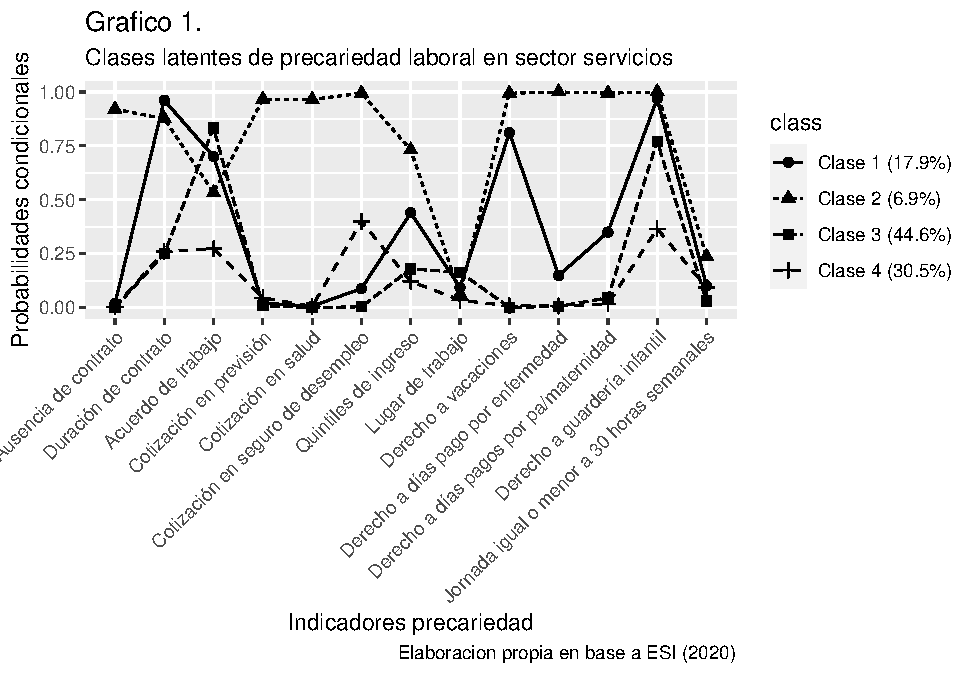
\includegraphics{informe_files/figure-latex/model_graph-1.pdf}

\hypertarget{tablas-cruzadas}{%
\subsection{Tablas cruzadas}\label{tablas-cruzadas}}

La \emph{tabla 4} da cuenta de la distribución de los individuos en cada
clase de precariedad laboral según sexo.Para empezar, la \emph{clase
subcontratada inestable} se compone mayoritariamente por hombres (67,5
\%), siendo las mujeres un 32,5 \%. Asimismo, la \emph{clase
multiprecarizada} presenta una mayor presencia masculina (76,1 \%),con
un 23,9\% de mujeres. En la misma línea, la \emph{clase subcontratada
protegida} posee un carácter masculinizado, en tanto 64,2\% de la clase
refiere a hombres y 35,8\% a mujeres. Finalmente, a diferencia del resto
de las clases previamente descritas, la \emph{clase de servicios
temporales protegida} se compone predominantemente por mujeres (76,7
\%), siendo los hombres sólo un 23,3\%. Cabe señalar que, a nivel global
entre las clases, más de la mitad de los hombres trabajadores del sector
servicios (56.2 \%) se concentran en la \emph{clase subcontratada
protegida}; mientras que casi la mitad de las mujeres trabajadoras (49.3
\%) pertenecen a la \emph{clase de servicios temporales protegida}.
Asimismo, el 35,7 \% de las mujeres trabajadoras del sector servicios
pertenecen a la \emph{clase de servicios temporales protegida}. Estos
hallazgos son interesantes, en tanto dan cuenta de que la posición de
los hombres en los empleos del sector servicios sería más precaria que
la de las mujeres durante el año 2019; sin embargo, no es posible
aseverar tal hallazgo sin considerar la fuerte salida de las mujeres del
mercado laboral con la pandemia. Necesariamente, quello abre la
interrogante sobre qué empleos del sector servicios fueron eliminados
con la pademia y cómo complementaría aquello los hallazgos aquí
presentados.

\begin{Shaded}
\begin{Highlighting}[]
\CommentTok{\#Asginar la clase de precariedad a cada sujeto}
\NormalTok{base\_proc }\OtherTok{\textless{}{-}} \FunctionTok{cbind}\NormalTok{(base\_proc, lc4}\SpecialCharTok{$}\NormalTok{predclass) }

\CommentTok{\#Renombrar la variable de clase de precariedad}
\NormalTok{base\_proc }\OtherTok{\textless{}{-}}\NormalTok{ base\_proc }\SpecialCharTok{\%\textgreater{}\%} \FunctionTok{rename}\NormalTok{(}\AttributeTok{Clase=}\StringTok{\textasciigrave{}}\AttributeTok{lc4$predclass}\StringTok{\textasciigrave{}}\NormalTok{)}

\CommentTok{\#Creación de tabla cruzada para variable sexo}
\FunctionTok{sjt.xtab}\NormalTok{(base\_proc}\SpecialCharTok{$}\NormalTok{Clase, base\_proc}\SpecialCharTok{$}\NormalTok{sexo, }
         \AttributeTok{title =} \StringTok{"Tabla 4.}
\StringTok{         Proporciones por clase de precariedad y sexo"}\NormalTok{,}
         \AttributeTok{show.row.prc =}\NormalTok{ T,}
         \AttributeTok{show.col.prc =}\NormalTok{ T)}
\end{Highlighting}
\end{Shaded}

Tabla 4. Proporciones por clase de precariedad y sexo

Clase

Sexo

Total

Hombre

Mujer

1

{280}{67.5~\%}{20.8~\%}

{135}{32.5~\%}{11.4~\%}

{415}{100~\%}{16.4~\%}

2

{134}{76.1~\%}{9.9~\%}

{42}{23.9~\%}{3.6~\%}

{176}{100~\%}{7~\%}

3

{758}{64.2~\%}{56.2~\%}

{422}{35.8~\%}{35.7~\%}

{1180}{100~\%}{46.6~\%}

4

{177}{23.3~\%}{13.1~\%}

{583}{76.7~\%}{49.3~\%}

{760}{100~\%}{30~\%}

Total

{1349}{53.3~\%}{100~\%}

{1182}{46.7~\%}{100~\%}

{2531}{100~\%}{100~\%}

χ2=402.049 · df=3 · Cramer's V=0.399 · p=0.000

El desglose del análisis de clases a partir del nivel educacional
contenido en la \emph{tabla 5} arroja que \emph{Educación secundaria} es
la categoría de mayor proporción dentro de las cuatro clases. Para la
\emph{clase subcontratada inestable}, esta categoría representa el
56,4\%, seguida por quienes poseen educación primaria (nivel 1 y 2) con
un 22,7\%, \emph{Educacion tecnica} con un 13\%, y \emph{Educacion
universitaria} con un 7,2\% . Para la \emph{clase multiprecarizada}, las
cifras se concentran en los primeros niveles educativos, donde
\emph{Educacion primaria (nivel 1)} reune un 13,6\% de los casos,
\emph{Educacion primaria (nivel 2)} un 27,3\%, y \emph{Educacion
secundaria} un 51,7\%. \emph{Educacion tecnica} y \emph{Educacion
universitaria} solo alcanzan un 3,4\% y un 4,5\% del total
respectivamente. Por su parte, la \emph{clase subcontratada protegida}
es aquella que concentra el mayor porcentaje de su total en la categoría
\emph{Educacion secundaria}, con un 62,9\%, siguiendo \emph{Educacion
técnica} y \emph{Educacion primaria (nivel 2)}, ambas con 11,9\%, luego
\emph{Educacion universitaria} con 6,6\%, y \emph{Educacion primaria
(nivel 1)} con un 6,4\%. Finalmente, la \emph{clase de servicios
temporales protegida} es aquella con mayores porcentajes de educación
superior, sumando un 47\% entre \emph{Educacion tecnica} y
\emph{Educacion universitaria} (con mayor proporción de la primera, con
un 30,4\% de los casos). Además, es la única clase con una proporción
mayor a cero de \emph{Postitulos y maestria} (1,3\%), pese a que este
porcentaje es aún muy reducido. Se sigue que para un 42,8\% de esta
clase su mayor nivel alcanzado es el secundario, y para un 8,8\% es el
primario (niveles 1 y 2).

\begin{Shaded}
\begin{Highlighting}[]
\CommentTok{\#Creación de tabla cruzada para variable educación}
\FunctionTok{sjt.xtab}\NormalTok{(base\_proc}\SpecialCharTok{$}\NormalTok{Clase, base\_proc}\SpecialCharTok{$}\NormalTok{educacion,}
         \AttributeTok{title =} \StringTok{"Tabla 5.}
\StringTok{         Proporciones por clase de precariedad y nivel educacional"}\NormalTok{,}
         \AttributeTok{show.row.prc =} \ConstantTok{TRUE}\NormalTok{)}
\end{Highlighting}
\end{Shaded}

Tabla 5. Proporciones por clase de precariedad y nivel educacional

Clase

Educacion

Total

Doctorado

Educacion primaria(nivel 1)

Educacion primaria(nivel 2)

Educacion secundaria

Educacion tecnica(superior nouniversitaria)

Educacionuniversitaria

Nunca estudio

Postitulos ymaestria

1

{0}{0~\%}

{33}{8~\%}

{61}{14.7~\%}

{234}{56.4~\%}

{54}{13~\%}

{30}{7.2~\%}

{3}{0.7~\%}

{0}{0~\%}

{415}{100~\%}

2

{0}{0~\%}

{24}{13.6~\%}

{48}{27.3~\%}

{90}{51.1~\%}

{6}{3.4~\%}

{8}{4.5~\%}

{0}{0~\%}

{0}{0~\%}

{176}{100~\%}

3

{0}{0~\%}

{75}{6.4~\%}

{140}{11.9~\%}

{742}{62.9~\%}

{140}{11.9~\%}

{78}{6.6~\%}

{4}{0.3~\%}

{1}{0.1~\%}

{1180}{100~\%}

4

{0}{0~\%}

{26}{3.4~\%}

{41}{5.4~\%}

{325}{42.8~\%}

{231}{30.4~\%}

{126}{16.6~\%}

{1}{0.1~\%}

{10}{1.3~\%}

{760}{100~\%}

Total

{0}{0~\%}

{158}{6.2~\%}

{290}{11.5~\%}

{1391}{55~\%}

{431}{17~\%}

{242}{9.6~\%}

{8}{0.3~\%}

{11}{0.4~\%}

{2531}{100~\%}

χ2=NaN · df=21 · Cramer's V=NaN · Fisher's p=0.000

Sobre la distribución etaria según cada una de las clases de
precariedad, en la \emph{tabla 6} se indica que la clase subcontratada
inestable (Clase 1) se compone casi la mitad (48,8 \%) de trabajadores
entre los 25 a 49 años. Asimismo, alrededor de un cuarto de dicha clase
se encuentra en el tramo etario entre los 20 hasta 29 años, mientras que
un quinto de este grupo (20,5 \%) tiene entre 50 a 64 años. El 6,4 \%
restante de la clase se distribuye en iguales proporciones entre los
tramos de 15 a 19 años y 65 años o más. En cuanto a la clase
multiprecarizada (Clase 2), un 48,4\% se encuentra en el tramo entre los
25 a 49 años, al mismo tiempo que más de un tercio (31,2 \%) tiene entre
50 a 64 años. Ambos tramos etarios concentran al 79,6 \% de trabajadores
de esta clase. Además, menos de un quinto del grupo (19,3 \%) se
encuentra entre los 20 y 29 años de edad, mientras que un 5,1 \% tiene
65 años o más y sólo un 3 \% entre 15 a 19 años. Por su parte, un 43,1
\% de la clase subcontrata protegida (Clase 3) se encuentra en el tramo
entre los 25 a 49 años, mientras que más de un tercio (34,7 \%) tiene
entre 50 a 64 años. En cuanto a la población entre los 20 a 29 años de
edad, esta se compone por menos de un quinto de la clase (17,2 \%). De
esta forma, el tramo entre los 65 años o más agrupa al 4,1 \% del grupo,
restando sólo un 1 \% de trabajadores entre los 15 a 19 años. Por
último, casi la mitad (48,6 \%) de la clase de servicios temporales
(Clase 4) tiene entre 25 a 49 años de edad, con más de un tercio (33,7
\%) de trabajadores en el tramo entre los 50 a 64 años. Asimismo, un
12,9 \% de la clase se encuentra entre los 20 a 29 años, con un 4,6 \%
de personas con 65 años o más y un 0,3 \% del grupo entre los 15 a 19
años.

\begin{Shaded}
\begin{Highlighting}[]
\CommentTok{\#Creación de tabla cruzada para variable edad}
\FunctionTok{sjt.xtab}\NormalTok{(base\_proc}\SpecialCharTok{$}\NormalTok{Clase, base\_proc}\SpecialCharTok{$}\NormalTok{edad,}
         \AttributeTok{title =} \StringTok{"Tabla 6.}
\StringTok{         Proporciones por clase de precariedad y edad"}\NormalTok{,}
         \AttributeTok{show.row.prc =}\NormalTok{ T,}
         \AttributeTok{encoding =} \StringTok{\textquotesingle{}UTF{-}8\textquotesingle{}}\NormalTok{)}
\end{Highlighting}
\end{Shaded}

Tabla 6. Proporciones por clase de precariedad y edad

Clase

Edad

Total

15 a 19 anos

20 a 29 anos

25 a 49 anos

50 a 64 anos

65 anos o mas

1

{14}{3.4~\%}

{101}{24.3~\%}

{201}{48.4~\%}

{85}{20.5~\%}

{14}{3.4~\%}

{415}{100~\%}

2

{3}{1.7~\%}

{34}{19.3~\%}

{75}{42.6~\%}

{55}{31.2~\%}

{9}{5.1~\%}

{176}{100~\%}

3

{12}{1~\%}

{203}{17.2~\%}

{508}{43.1~\%}

{409}{34.7~\%}

{48}{4.1~\%}

{1180}{100~\%}

4

{2}{0.3~\%}

{98}{12.9~\%}

{369}{48.6~\%}

{256}{33.7~\%}

{35}{4.6~\%}

{760}{100~\%}

Total

{31}{1.2~\%}

{436}{17.2~\%}

{1153}{45.6~\%}

{805}{31.8~\%}

{106}{4.2~\%}

{2531}{100~\%}

χ2=69.238 · df=12 · Cramer's V=0.095 · Fisher's p=0.000

\hypertarget{conclusiones}{%
\section{Conclusiones}\label{conclusiones}}

A partir del análisis de la medida de ajuste de los modelos de clases
latentes elaborados, que contemplaron entre 1 y 12 clases, se optó por
el modelo de 4 clases, que incluye la denominada \emph{clase de
servicios temporales protegida}, que corresponde a un 30\% del total de
trabajadores del sector servicios, con alta probabilidad de poseer
contratos indefinidos y, en general, condiciones laborales e ingresos no
precarios. Es así como puede señalarse que se cumple la primera
hipótesis planteada.

En relación con la segunda hipótesis, es posible señalar que esta no se
cumple del todo. En efecto, la \emph{clase de servicios temporales
protegida} es la única que presenta una mayor proporción de
trabajadoras. Las clases \emph{multiprecarizada} y \emph{subcontratada
protegida}, a su vez, presentan un carácter masculinizado. A nivel
global, más de la mitad de los trabajadores masculinos del sector
servicios se concentran en la clase subcontratada protegida; mientras
que casi la mitad de las mujeres trabajadoras pertenecen a la clase de
servicios temporales protegida. No obstante, hay que considerar el
retroceso de aproximadamente 10 años en términos de la inserción laboral
de las mujeres producido por la crisis sanitaria: es probable que gran
parte de las trabajadoras cuya inserción laboral tuviese un carácter más
precario se encontrasen desocupadas al momento de la medición. Junto con
ello, la crisis de los cuidados - engrandecida por la pandemia - también
puede haber sido un elemento que restase a la fuerza de trabajo femenina
perteneciente a las clases más precarias.

La clase \emph{subcontratada inestable} presenta una alta proporción de
trabajadores cuyo nivel educacional es igual o inferior a la educación
secundaria. Lo mismo sucede con la \emph{clase multiprecarizada}. En
ambos casos, la proporción de trabajadores cuyo nivel educacional es
universitario o superior es inferior al 10\%. La clase \emph{de
servicios temporales protegida}, por su parte, es la que concentra el
mayor porcentaje de trabajadores con un nivel educacional técnico y
universitario. Así, se cumple la tercera hipótesis planteada.

Por último, casi un 25\% de los trabajadores pertenecientes a la clase
\emph{subcontratada inestable} tiene una edad inferior a 29 años.
Asimismo, un 20\% de los trabajadores pertenecientes a esta clase tienen
una edad cercana a la jubilación. La clase \emph{multiprecarizada}, por
su parte, también se concentra cerca de un quinto trabajadores con menos
de 29 años; y en torno a un tercio de los trabajadores que se integran a
esta clase se encuentran cerca de la edad de jubilación. No obstante, la
distribución etaria para todas las clases (incluyendo aquellas con
mayores niveles de protección) es similar, por lo cual puede sostenerse
que no es posible concluir que quienes tienen menos de 30 años, o
quienes se encuentran prontos a jubilar, están insertados de manera más
precaria en el mercado del trabajo chileno.

En base a lo anterior, es posible cumplir el objetivo general que guía a
esta investigación: a saber, determinar la distribución de los
diferentes tipos de precariedad laboral de trabajadoras y trabajadores
en el sector servicios en 2020 en Chile, según sexo, edad, edad y nivel
educacional.

No obstante, hay todavía muchos elementos que valdría la pena investigar
en torno a la precarización laboral en Chile desde una perspectiva
multidimensional. Entre ellos, valdría la pena analizar el resto de los
sectores de la economía (industrias manufactureras y de extracción de
materias primas), así como establecer comparaciones de los niveles de
precariedad de estos respecto del sector de servicios, analizado en esta
investigación. También sería interesante analizar, por ejemplo, el
acceso a transferencias proveídas por el Estado durante la pandemia -
como el Ingreso Familiar de Emergencia, entre otros - para cada una de
las clases aquí presentadas. También podría resultar de sumo interés
científico y público preguntarse por la relación entre estas clases y el
tiempo dedicado al trabajo no remunerado, entre otros.

\hypertarget{referencias}{%
\section*{Referencias}\label{referencias}}
\addcontentsline{toc}{section}{Referencias}

\hypertarget{refs}{}
\begin{CSLReferences}{1}{0}
\leavevmode\hypertarget{ref-aguiar2010}{}%
Aguiar, S. (2010). El grado de flexiprecariedad en el trabajo. {El}
proceso de innovación y la relación capital-trabajo. \emph{Tesis
Magister Ciencias Sociales}.

\leavevmode\hypertarget{ref-antunes2005}{}%
Antunes, R. (2005). \emph{Los sentidos del trabajo: Ensayo sobre la
afirmación y la negación del trabajo}. Herramienta.

\leavevmode\hypertarget{ref-anxo2017}{}%
Anxo, D., Baird, M., \& Erhel, C. (2017). Work and care regimes and
women's employment outcomes. In D. Grimshaw, C. Fagan, G. Hebson, \& I.
Tavora (Eds.), \emph{Making work more equal}. Manchester University
Press. \url{https://doi.org/10.7765/9781526125972.00025}

\leavevmode\hypertarget{ref-arriagada2007}{}%
Arriagada, I. (2007). \emph{Abriendo la caja negra del sector servicios
en {Chile} y {Uruguay}}. CLACSO.
\url{http://bibliotecavirtual.clacso.org.ar/clacso/gt/20101012013122/03Arriagada.pdf}

\leavevmode\hypertarget{ref-blanco2019}{}%
Blanco, O., \& Julian, D. (2019). \emph{Una tipología de precariedad
laboral para {Chile}: La precariedad como fenómeno transclasista}.
\emph{129}.

\leavevmode\hypertarget{ref-boccardo2020}{}%
Boccardo, G. (2020). \emph{{TRABAJAR} {EN} {TIEMPOS} {DE} {PANDEMIA}:
¿{ANTESALA} {DE} {NUESTRO} {FUTURO} {LABORAL}?} \emph{17}.

\leavevmode\hypertarget{ref-instituonacionaldeestadisticas2020}{}%
Estadísticas, I. N. de. (2020). \emph{Documento {Metodológico}
{Encuesta} {Nacional} de {Empleo} ({ENE})}. 129.

\leavevmode\hypertarget{ref-instituonacionaldeestadisticas2021}{}%
Estadísticas, I. N. de. (2021). \emph{Documento {Metodológico}
{Encuesta} {Suplementaria} de {Ingresos}, {ESI} 2020}.

\leavevmode\hypertarget{ref-guadagni1964}{}%
Guadagni, A. A. (1964). La {Estructura} {Ocupacional} y el {Desarrollo}
{Economico} de {Chile}. \emph{Journal of Inter-American Studies},
\emph{6}(2), 187--201.

\leavevmode\hypertarget{ref-hagenaars2002}{}%
Hagenaars, J. A., \& McCutcheon, A. L. (2002). \emph{Applied {Latent}
{Class} {Analysis}}. 478.

\leavevmode\hypertarget{ref-julian2014}{}%
Julian, D. (2014). \emph{La precariedad laboral, modernidad y
modernización capitalista: {Una} contribución al debate desde {América}
{Latina}}. \emph{23}.

\leavevmode\hypertarget{ref-julian2020}{}%
Julian, D. (2020). \emph{Precariedad como gobierno de la pandemia: {La}
experiencia de la precariedad laboral en {Chile}}. \emph{11}, 125--149.

\leavevmode\hypertarget{ref-lazarocastellanos2017}{}%
Lázaro Castellanos, R., \& Jubany Baucells, O. (2017).
\emph{Interseccionalidad del género y mercado de trabajo postfordista}.
\emph{5}(46).

\leavevmode\hypertarget{ref-linzer2011}{}%
Linzer, D. A., \& Lewis, J. B. (2011). \textbf{poLCA} : {An} \emph{r}
{Package} for {Polytomous} {Variable} {Latent} {Class} {Analysis}.
\emph{J. Stat. Soft.}, \emph{42}(10).
\url{https://doi.org/10.18637/jss.v042.i10}

\leavevmode\hypertarget{ref-marchetti2020}{}%
Marchetti, P. (2020). Empleo informal como "estrategia de
sobrevivencia": {Expertos} prevén alzas y urgen por políticas para
combatirlo. In \emph{Emol}.
\url{https://www.emol.com/noticias/Economia/2020/08/28/996237/Informalidad-Chile-pandemia-expertos-politicasformalizar.html}

\leavevmode\hypertarget{ref-mora2010}{}%
Mora, M. (2010). \emph{Ajuste y empleo: La precarización del trabajo
asalariado en la era de la globalización} (1a. ed). Colegio de México.

\leavevmode\hypertarget{ref-perez2019}{}%
Pérez, C. (2019). Verónica {Schild}: "{El} secreto de la economía
chilena es la mano de obra precaria feminizada" {[}El
\{Desconcierto\}{]}. In \emph{El Desconcierto}.
\url{https://www.eldesconcierto.cl/2019/12/04/veronica-schild-el-secreto-de-la-economia-chilena-es-la-mano-de-obra-precaria-feminizada/}

\leavevmode\hypertarget{ref-ravest2016}{}%
Ravest, J. (2016). \emph{La fisonomía del sector servicios en {Chile}.
{Avances} y proyecciones respecto del {``{Trabajo} {Decente}.''}}
Departamento de Sociología Universidad de Chile.

\leavevmode\hypertarget{ref-schonhaut2020}{}%
Schönhaut, C. (2020). Trabajos feminizados en la pandemia: Remunerados y
no remunerados. \emph{El Desconcierto}.
\url{https://www.eldesconcierto.cl/2020/04/12/trabajos-feminizados-en-la-pandemia-remunerados-y-no-remunerados/}

\leavevmode\hypertarget{ref-semenza2021}{}%
Semenza, R., Boccardo, G., \& Sarti, S. (2021). So {Far}, so {Similar}?
{Labour} {Market} {Feminization} in {Italy} and {Chile}. \emph{Soc Indic
Res}, \emph{154}(3), 917--942.
\url{https://doi.org/10.1007/s11205-020-02551-0}

\leavevmode\hypertarget{ref-standing1999}{}%
Standing, G. (1999). Global {Feminization} {Through} {Flexible} {Labor}:
{A} {Theme} {Revisited}. \emph{World Development}, \emph{27}, 583--602.
\url{https://citeseerx.ist.psu.edu/viewdoc/download?doi=10.1.1.1077.7385\&rep=rep1\&type=pdf}

\leavevmode\hypertarget{ref-weller2020}{}%
Weller, B. E., Bowen, N. K., \& Faubert, S. J. (2020). Latent {Class}
{Analysis}: {A} {Guide} to {Best} {Practice}. \emph{Journal of Black
Psychology}, \emph{46}(4), 287--311.
\url{https://doi.org/10.1177/0095798420930932}

\leavevmode\hypertarget{ref-weller2001}{}%
Weller, J. (2001). \emph{Procesos de exclusión e inclusión laboral: La
expasión del empleo en el sector terciario}. Naciones Unidas, CEPAL,
División de Desarrollo Económico.

\leavevmode\hypertarget{ref-weller2004}{}%
Weller, J. (2004). \emph{El empleo terciario en {América} {Latina}:
Entre la modernidad y la sobrevivencia}. Revista de la CEPAL No.84.

\end{CSLReferences}

\end{document}
